% Shared preamble for the CIG-AMF formal-research papers.
% IEEEtran conference class; compiles on Overleaf without modification.
\documentclass[conference]{IEEEtran}
\IEEEoverridecommandlockouts

\usepackage{cite}
\usepackage{amsmath,amssymb,amsfonts}
\usepackage{amsthm}
\usepackage{algorithm}
\usepackage{algorithmic}
\usepackage{graphicx}
\usepackage{textcomp}
\usepackage{xcolor}
\usepackage{booktabs}
\usepackage{url}
\usepackage[hidelinks]{hyperref}

\def\BibTeX{{\rm B\kern-.05em{\sc i\kern-.025em b}\kern-.08em T\kern-.1667em\lower.7ex\hbox{E}\kern-.125emX}}

\newtheorem{theorem}{Theorem}
\newtheorem{lemma}[theorem]{Lemma}
\newtheorem{proposition}[theorem]{Proposition}
\newtheorem{corollary}[theorem]{Corollary}
\theoremstyle{definition}
\newtheorem{definition}[theorem]{Definition}
\newtheorem{remark}[theorem]{Remark}
\newtheorem{example}[theorem]{Example}

% A machine-checked statement carries its Lean declaration name.
\newcommand{\lean}[1]{\textsf{\footnotesize #1}}
\newcommand{\leanbox}[1]{%
  \par\vspace{2pt}\noindent
  {\footnotesize\textsf{Lean: #1}}\par\vspace{2pt}}

% Evidence classes, used consistently and never interchangeably.
\newcommand{\PROVED}{\textsc{proved}}
\newcommand{\CERT}{\textsc{certificate}}
\newcommand{\NUM}{\textsc{numerical}}
\graphicspath{{../_figures/}}


\begin{document}

\title{The Information Cost of a Compression Decision\\
under Support and Measurement Constraints}

\author{\IEEEauthorblockN{Vu Phan An Nguyen}
\IEEEauthorblockA{\textit{Rider University} \\
Lawrenceville, NJ, USA}}

\maketitle

\begin{abstract}
Six strands of this programme have been developed against separate models: an exchange
bound for retained-coordinate compression, a certificate geometry for the alternatives
that make a compression wrong, a support-restricted loss, a query calculus, a calibration
model, and a constrained-ranking optimum. This paper puts them in one question---given the
measurements we are allowed and the constraints on what we may serve, what does it cost to
find a compression whose regret is at most $\varepsilon$?---and reports what changes when
they meet. Three things change, and each is a statement rather than a reframing. First, the
support is an independent variable: we give an identity decomposing a support-restricted
comparison into a full-domain comparison plus a geometry term, an exchange bound that
carries the term, and a three-coordinate witness with \emph{zero} interaction on which the
Top-$C$ rule is optimal on the cube and worst on the support, with the corrected inequality
holding with equality. Second, certifying a margin is strictly more expensive than making
the decision the margin is used to justify: on a two-coordinate family the decision depends
only on $a-b$ while the certificate compares $a-b$ against $2c$, and the computed cost
ratio reaches $1089$ before the certificate becomes unattainable at any cost while the
decision remains settled. Third, we study a combinatorial obstruction criterion for deciding without identifying:
we prove that a grouping of worlds admits a common safe answer if and only if no
obstruction lies inside a class, and that every randomised rule leaves unsafe mass at least
$1/|H|$ somewhere in an obstruction $H$. Along one deformation of the witness we compute
the exact information game for an $\varepsilon$-correct compression under a nuisance
offset, $\Gamma_{\rm comp}=9\Delta_{\rm dec}^{2}/2(\sigma\sqrt{c_{o}}+\nu\sqrt{c_{a}})^{2}$
with $\Delta_{\rm dec}=|\theta-\tfrac34|+\varepsilon/2$, and identify a phase in which the
optimal design measures nothing. We also show the geometry term is measurable from $2m$ oscillations---and that the
criterion this yields is vacuous, firing $0$ times in $919$ trials, while the exact constant
fires but costs $\binom{m}{k}$ evaluations and its cheap single-swap surrogate is unsound.
Six Lean~4 modules carry the new statements; the mechanisms we do \emph{not} claim as new,
and the places where our own bounds are weak, are stated as such.
\end{abstract}

\begin{IEEEkeywords}
compression, support geometry, information lower bounds, experimental design, formal
verification
\end{IEEEkeywords}

\section{Introduction}
\label{sec:intro}

\subsection{One question}

Each strand of this programme answers a question of the form ``what is the right
compression, and how would we know?'' but each answers it against its own model. Put them
in a single question and the models have to agree:

\begin{quote}
\emph{Given the measurements we are permitted and the constraints on what we may serve,
what does it cost to find a compression decision whose regret is at most $\varepsilon$?}
\end{quote}

Write $F$ for the world, $K$ for the support on which the compression must be good, $d$ for
the decision returned, $\mathcal{D}$ for the admissible decisions, $R_{F}(d)$ for the true
regret, $P^{q}_{F,b}$ for the law of query $q$ in the presence of a nuisance $b$, and
$c_{q}$ for the cost of $q$. Then the six strands occupy the places shown in
Table~\ref{tab:roles}.

\begin{table}[t]
\caption{Where each strand enters the common problem.}
\label{tab:roles}
\centering
\footnotesize
\begin{tabular}{@{}ll@{}}
\toprule
Strand & Role \\
\midrule
D6 & response ranking, interaction, and regret \\
Functional & geometry of the alternatives that make $d$ wrong \\
Support & the support $K$, and worlds sharing a safe answer \\
Query & which worlds a measurement separates, and how fast \\
MASTER & nuisance and calibration \\
Structural & constraints on the served decision \\
\bottomrule
\end{tabular}
\end{table}

One distinction is maintained throughout and is not cosmetic. \emph{Structural} constrains
the decision that is served---one ranking, a menu, prescribed marginals. \emph{Allocation}
constrains the data that is gathered. Both are expressible with permutations and budgets
and they are not the same object; a result about one is not a result about the other.

The target is to separate three regimes:
\begin{equation}
\begin{aligned}
&\text{no feasible decision}\\
&\quad\to\;\text{feasible but uninformed}\\
&\qquad\to\;\text{learnable at finite cost.}
\end{aligned}
\label{eq:regimes}
\end{equation}
Defining these regimes is not itself a contribution. The thresholds and costs below are.

\subsection{What is claimed, and what is not}

We separate three kinds of statement and never let them blur.

\textbf{Proved in Lean.} The support decomposition identity and its exchange bound; the
$\kappa$-threshold; the witness in which Top-$C$ fails on a support with zero interaction
and the corrected bound holds with equality; the loss curves, flip point, safe intervals
and $\Delta_{\rm dec}$ of the deformed family; the nuisance-profiling and allocation steps
of the information game; the moment-vanishing law for bounded low-degree queries; the
obstruction--class equivalence and the randomised error floor; the relaxed-marginal
lower bound for Structural. Module names appear in \leanbox{} boxes at each statement.

\textbf{Exact finite arithmetic versus numerical diagnostics.} The tested moment
identities and support-witness losses use rational arithmetic. The Structural frontier
uses floating-point LP optimization; certificate costs use numerical optimization; Hellinger
values use numerical quadrature. No exact optimizer certificate is supplied. The obstruction
script assigns order indices separately from its compression span vectors, so it is a
combinatorial diagnostic, not a common-model rate proof.

\textbf{Not claimed as new.} Several mechanisms here have close prior art and we use them
as tools. Information max--min formulations with several correct answers are developed by
Degenne and Koolen~\cite{degenne2019}; controlled sensing with non-uniform costs by
Nitinawarat and Veeravalli~\cite{nitinawarat2013}; the fact that increasing hidden interaction order at fixed measurement degree
can postpone the first informative moment, and with it the sample cost, is exactly the
masking mechanism analysed by Grosso, Standaert and Prouff~\cite{grosso2014}, with
moment-expansions of information in the side-channel setting given by Rioul, Cheng and
Guilley~\cite{rioul2021}; randomised rankings with probability constraints on prefix
membership are the subject of Singh, Kempe and Joachims~\cite{singh2021} and
Singh and Joachims~\cite{singh2018}; and deciding without identifying, via overlapping
decision regions, is due to Javdani et al.~\cite{javdani2014}. We do not present any of
these as discoveries. What we offer are the specific laws in which our components appear
\emph{together}, and the quantitative gaps they produce.

\NOTEPAR{The honest summary of novelty for the final version: the contribution is not any
single mechanism but that replacing one component changes the same final optimum,
threshold or rate. The support term in the exchange bound, the certificate/decision cost
separation, the $\eta$-frontier breakpoints, and the obstruction order law are the four
places where that is demonstrated quantitatively. Everything else is scaffolding.}

\section{The support is an independent variable}
\label{sec:support}

\subsection{Setting}

Let $X$ be the full product domain and $K\subseteq X$ the support on which the compression
must be good. For a retained set $T$ let $r_{T}$ be the residual after retaining $T$, and
define the losses by the oscillation of the residual on each domain,
\begin{equation}
L_{X}(T)=\tfrac12\operatorname{osc}_{X}r_{T},\qquad
L_{K}(T)=\tfrac12\operatorname{osc}_{K}r_{T}.
\label{eq:twolosses}
\end{equation}
Because $K\subseteq X$, the oscillation is monotone in the domain, so
\begin{equation}
D_{K}(T)\;=\;L_{X}(T)-L_{K}(T)\;\ge\;0 ,
\label{eq:gap}
\end{equation}
the part of the loss the support removes.

\leanbox{\lean{geomGap\_nonneg} and \lean{osc\_eq\_oscOn\_univ} in
\lean{LeanUnifiedSupportExchangeV1}}

The second name matters: it identifies the full domain with the support $K=X$, so the
support-restricted statement and the unrestricted one are about the same object rather
than being analogous.

\subsection{The decomposition and the exchange bound}

\begin{theorem}[Support decomposition]
\label{thm:decomp}
For all residuals and all $T,S$,
\begin{equation}
L_{K}(T)-L_{K}(S)=\bigl(L_{X}(T)-L_{X}(S)\bigr)+\bigl(D_{K}(S)-D_{K}(T)\bigr).
\label{eq:identity}
\end{equation}
\end{theorem}

\leanbox{\lean{support\_decomposition} in \lean{LeanUnifiedSupportExchangeV1}}

Equation~\eqref{eq:identity} is an identity, not a bound: everything the support does to a
comparison is carried by the two gap terms and the full-domain difference is untouched.
Feeding any full-domain exchange bound through it gives the support version.

\begin{theorem}[Exchange on a support]
\label{thm:supportexchange}
With $T$ Top-$C$ by the oscillation score, margin $\rho$ and interaction bound
$\delta_{I}$,
\begin{equation}
2\bigl[L_{K}(T)-L_{K}(S)\bigr]\le|T\setminus S|\,(2\delta_{I}-\rho)
+2\bigl[D_{K}(S)-D_{K}(T)\bigr].
\label{eq:supportexchange}
\end{equation}
\end{theorem}

\leanbox{\lean{support\_exchange\_of\_full} in \lean{LeanUnifiedSupportExchangeV1}}

\begin{corollary}[Threshold]
\label{cor:kappa}
Assume the full-domain exchange theorem applies, with nonnegative interaction bound,
and $D_{K}(S)-D_{K}(T)\le\kappa|T\setminus S|$ for every competitor $S$ with $|S|=|T|$.
Then
\begin{equation}
\rho\;\ge\;2\delta_{I}+2\kappa\quad\Longrightarrow\quad T\ \text{is optimal on}\ K .
\label{eq:kappathreshold}
\end{equation}
\end{corollary}

\leanbox{\lean{support\_optimal\_of\_margin} in \lean{LeanUnifiedSupportExchangeV1}}

At $\kappa=0$ this is the unrestricted threshold unchanged, so the law degrades correctly
when the support is the whole domain.

\subsection{The witness: zero interaction, wrong answer}

Take
\begin{equation}
\begin{aligned}
F(x)&=3x_{1}-2x_{2}-2x_{3},\\
X&=\{0,1\}^{3},\qquad K=\{000,111\},
\end{aligned}
\label{eq:witness}
\end{equation}
with a corner reference. Then $F$ is additive, so $\delta_{I}=0$ and every hypothesis of
the unrestricted exchange theorem holds in its strongest form. The component spans are
$C=(3,2,2)$, so Top-$C$ at $k=1$ retains coordinate~$1$ with margin $\rho=1$. The four
losses are
\begin{equation}
\begin{aligned}
L_{X}(\{1\})&=2, & L_{X}(\{2\})&=\tfrac52,\\
L_{K}(\{1\})&=2, & L_{K}(\{2\})&=\tfrac12 .
\end{aligned}
\label{eq:witnesslosses}
\end{equation}
On the cube Top-$C$ is right. On the support it is the \emph{worst} of the three
singletons. The gaps are $D_{K}(\{1\})=0$ and $D_{K}(\{2\})=2$, and that asymmetry is the
failure.

\begin{theorem}[The geometry term is not slack]
\label{thm:equality}
At the witness, the doubled support regret is $3$; the plain full-domain bound asserts it
is at most $-1$ and is therefore false on $K$; and \eqref{eq:supportexchange} holds with
\emph{equality}.
\end{theorem}

\leanbox{\lean{witness\_plain\_bound\_fails} and \lean{witness\_exchange\_equality} in
\lean{LeanUnifiedSupportExchangeV1}}

Equality is the point. A proof that dropped the geometry term would be proving something
false, so the term cannot be removed by a better argument. The witness also shows that
$\kappa$ is not controlled by the interaction: here $\delta_{I}=0$ while $\kappa=2$, so the
threshold demands $\rho\ge4$ against an actual margin of $1$.

\subsection{The geometry term is measurable}

Corollary~\ref{cor:kappa} would be a bridge and not a result if $\kappa$ stayed an input,
so we examine a bound in the ADDITIVE omitted-component model. For this model the gap
splits into two measurable pieces,
\begin{equation}
D_{K}(T)=\tfrac12\Bigl[\sum_{j\notin T}(s_{j}-c_{j})+\gamma_{K}(T^{\complement})\Bigr],
\label{eq:gapsplit}
\end{equation}
where $s_{j}$ and $c_{j}$ are coordinate $j$'s response oscillations on the full domain and
on the support, and
$\gamma_{K}(A)=\sum_{j\in A}c_{j}-\operatorname{osc}_{K}\bigl(\sum_{j\in A}Q_{j}\bigr)\ge0$
is the \emph{support coupling defect}: the amount by which the coordinates fail to reach
their extremes simultaneously on $K$. On the full domain the defect vanishes---that is
modularity---so $D_{K}$ is carried entirely by how much the support narrows each coordinate
and correlates them.

\leanbox{\lean{geomGap\_eq\_of\_modular} in \lean{LeanUnifiedGeometryBoundV1}}

\begin{theorem}[A computable geometry rate]
\label{thm:kappabound}
$\displaystyle D_{K}(S)-D_{K}(T)\;\le\;\tfrac12\sum_{j\in T\setminus S}(s_{j}+c_{j})$,
so any $\kappa$ dominating $(s_{j}+c_{j})/2$ on $T$ is a valid geometry rate.
\end{theorem}

\leanbox{\lean{geomGap\_diff\_le\_spans}, \lean{kappa\_of\_spans},
\lean{computable\_threshold} in \lean{LeanUnifiedGeometryBoundV1}}

The competitor's own coordinates contribute nothing, because a support span never exceeds a
full span. The bound uses $2m$ span values and covers every competitor in this additive model.
A span needs a certified range oracle or complete extrema calculation; it is not one
point, membership, or noisy query. Product reference alone does not make the actual
residual $F-\sum_{j\in T}Q_j$ equal to the omitted-component residual.

\subsection{...and the criterion built from it is nevertheless vacuous}

We report what that bound is worth, which is little. On $919$ random additive families with
random supports the resulting threshold fired \emph{zero} times. The obstruction is algebraic: the genuine margin gives $\rho+s_j\le s_i$ for
$i\in T,j\notin T$, while the span certificate gives
$2\delta_I+s_i+c_i\le2\delta_I+2\kappa\le\rho$. Thus
$2\delta_I+c_i+s_j\le0$. Nonnegative terms must all vanish; for nonempty $T$ and
complement this forces zero support spans and zero additive support loss. This is stronger
than a zero firing count on a numerical panel.

The exact constant---the largest rate over \emph{every} competitor of the given size---does
fire, on $779$ of the same $919$ instances, concentrated where the support is large. But it
costs $\binom{m}{k}$ support evaluations. The obvious cheap surrogate, maximising over
single swaps only at cost $O(m^{2})$, is \emph{unsound} once the budget exceeds one: a
competitor may differ from $T$ in several coordinates, and the same run exhibits instances
where it certifies a $T$ that is not optimal on the support. \NUM{}

\TODOPAR{This sharpens the open problem rather than closing it. It is no longer ``can
$\kappa$ be computed''---it can, expensively---but ``is there a polynomially computable
$\kappa$ strong enough to fire''. Theorem~\ref{thm:kappabound} shows the na\"ive span bound
is not, and the single-swap surrogate is not even sound. A route worth trying is to bound
the \emph{increment} of $\gamma_{K}$ under an exchange, rather than each coordinate's
contribution separately; the slack in Theorem~\ref{thm:kappabound} sits entirely in that
step. Do not describe the geometry rate as ``computable'' in the final version without this
qualification.}

\section{Certifying costs more than deciding}
\label{sec:oracle}

\subsection{Two different half-spaces}

The previous section's certificate asks for a margin. That is a stronger question than the
decision it justifies, and the gap is quantifiable. On the full cube take
\begin{equation}
F(x_{1},x_{2})=ax_{1}+bx_{2}+cx_{1}x_{2},\qquad a>b>0,\ c>0 ,
\label{eq:abc}
\end{equation}
with a corner reference. Then $L(\{1\})=(b+c)/2$ and $L(\{2\})=(a+c)/2$, so the
\emph{decision} is settled by the sign of $a-b$ alone, while $\delta_{I}=c$ and the Top-$C$
margin \emph{certificate} $\rho\ge2\delta_{I}$ reads $a-b\ge2c$. Both are half-space
questions about $\theta=(a,b,c)$, but about different half-spaces, and the certificate's
boundary is strictly closer to the truth whenever $c>0$.

\subsection{The cost of each}

Let observations be Gaussian and linear in $\theta$, with $q_{1}\mapsto a$,
$q_{2}\mapsto b$, $q_{3}\mapsto a+b+c$, unit variance and unit cost, and an allocation $w$
on the simplex. For a half-space alternative $\{\theta':v\cdot\theta'\le t\}$ the profiled
information is
\begin{equation}
\tfrac12\,(v\cdot\theta-t)^{2}\big/\bigl(v^{\mathsf T}W(w)^{-1}v\bigr),\qquad
W(w)=\textstyle\sum_{q}w_{q}M_{q}^{\mathsf T}M_{q},
\label{eq:halfspace}
\end{equation}
and the game value is its maximum over $w$. Table~\ref{tab:oraclegap} reports both games
at $a=3$, $b=1$, $\varepsilon=0.1$.

\begin{table}[t]
\caption{The cost of the margin certificate against the cost of the decision it justifies.
Computed by blind search over the allocation simplex; formula~\eqref{eq:halfspace} was
confirmed against direct constrained minimisation to a relative gap of $6.7\times10^{-4}$.
\NUM{}}
\label{tab:oraclegap}
\centering
\footnotesize
\begin{tabular}{@{}rrrr@{}}
\toprule
$c$ & $\Gamma_{\rm dec}$ & $\Gamma_{\rm cert}$ & cost ratio \\
\midrule
$0.05$ & $0.6050$ & $0.0501$ & $12.1$ \\
$0.25$ & $0.6050$ & $0.0313$ & $19.4$ \\
$0.50$ & $0.6050$ & $0.0139$ & $43.6$ \\
$0.75$ & $0.6050$ & $0.0035$ & $174.2$ \\
$0.90$ & $0.6050$ & $0.0006$ & $1089.0$ \\
$1.00$ & $0.6050$ & $0$ & $\infty$ \\
$1.50$ & $0.6050$ & $0$ & $\infty$ \\
\bottomrule
\end{tabular}
\end{table}

Two features deserve emphasis. The ratio is already three orders of magnitude at $c=0.9$,
well before anything degenerates; and at $a-b\le2c$ the true world itself fails the margin
condition, so the certificate is unattainable at \emph{any} cost while the decision remains
settled at $\Gamma_{\rm dec}=0.605$. That is a quantitative separation between learning the
decision and learning a sufficient certificate, on one family, with one query set and one
target regret.

\NOTEPAR{What is \emph{not} shown here: that the Top-$C$ margin is the best available
certificate. A weaker sufficient condition tailored to this family might close much of the
gap. The claim is about this certificate, which is the one the corpus actually uses.}

\section{Calibration on the same family}
\label{sec:calibration}

\subsection{A deformation with a flip point}

Deform the witness of Section~\ref{sec:support} along one parameter,
\begin{equation}
F_{\theta}(x)=(3+\theta)x_{1}+(-2+\theta)x_{2}+(-2+\theta)x_{3},\quad\theta\in[0,1],
\label{eq:thetafamily}
\end{equation}
keeping $K=\{000,111\}$. Evaluating the losses on the support,
\begin{equation}
L_{\theta}(\{1\})=2-\theta,\qquad L_{\theta}(\{2\})=L_{\theta}(\{3\})=\tfrac12+\theta,
\label{eq:thetalosses}
\end{equation}
so the right answer flips at
\begin{equation}
\theta_{*}=\tfrac34 .
\label{eq:flip}
\end{equation}
The flip point is a property of the geometry, not of any estimator.

\leanbox{\lean{loss\_retain\_first}, \lean{loss\_retain\_second},
\lean{decision\_flips\_at\_three\_quarters} in \lean{LeanUnifiedCompressionDecisionV1}}

An answer is $\varepsilon$-safe when its loss exceeds the best by at most $\varepsilon$.
The safe intervals are $[\tfrac34-\tfrac{\varepsilon}{2},\infty)$ for the first coordinate
and $(-\infty,\tfrac34+\tfrac{\varepsilon}{2}]$ for the second, so for the better answer
the distance to the nearest world at which it stops being safe is
\begin{equation}
\Delta_{\rm dec}(\theta,\varepsilon)=\Bigl|\theta-\tfrac34\Bigr|+\frac{\varepsilon}{2}.
\label{eq:deltadec}
\end{equation}

\leanbox{\lean{safe\_first\_iff}, \lean{safe\_second\_iff},
\lean{decision\_distance\_eq} in \lean{LeanUnifiedCompressionDecisionV1}}

\subsection{The nuisance, and why it costs money}

Allow two measurements, both on the support, both carrying a shared calibration offset $b$:
\begin{equation}
\begin{aligned}
Y&=F_{\theta}(111)+b+\xi=-1+3\theta+b+\xi, &\xi&\sim N(0,\sigma^{2}),\\
Z&=F_{\theta}(000)+b+\zeta=b+\zeta, &\zeta&\sim N(0,\nu^{2}),
\end{aligned}
\label{eq:measurements}
\end{equation}
at costs $c_{o}$ and $c_{a}$. The offset is a pure nuisance and $Y$ alone cannot see past
it: the worlds $(\theta,b)=(0,0)$ and $(1,-3)$ give $Y$ exactly the same law, yet demand
different answers whenever $\varepsilon<\tfrac12$. Only $Z$ breaks the confound, and $Z$
costs money; that is what makes this an allocation problem rather than an estimation
problem.

\leanbox{\lean{confounded\_pair\_same\_law} and
\lean{confounded\_pair\_need\_different\_answers} in
\lean{LeanUnifiedCompressionDecisionV1}}

\subsection{The game value}

Profiling the nuisance shift and optimising the allocation under
$c_{o}w_{o}+c_{a}w_{a}=1$ gives the value of the information game.

\begin{theorem}[Cost of an $\varepsilon$-correct compression]
\label{thm:gamma}
\begin{equation}
\Gamma_{\rm comp}(\theta,\varepsilon)
=\frac{9\,\Delta_{\rm dec}(\theta,\varepsilon)^{2}}
{2\bigl(\sigma\sqrt{c_{o}}+\nu\sqrt{c_{a}}\bigr)^{2}} .
\label{eq:gamma}
\end{equation}
\end{theorem}

\leanbox{\lean{nuisance\_profiled\_information}, \lean{allocation\_lower\_bound},
\lean{allocation\_optimum\_attained}, \lean{game\_value\_upper} in
\lean{LeanUnifiedCompressionDecisionV1}}

The two steps are proved separately: the inner minimisation over the nuisance shift is an
exact completed square, and the outer optimisation is a Cauchy--Schwarz step whose equality
case is the square-root allocation rule. Neither step is new. The completed square is
already in the corpus as \lean{LeanMasterCalibrationLawV1.profiled\_information}, in the
variables $(a,b,D)$; setting $a=w_{o}/2\sigma^{2}$ and $b=w_{a}/2\nu^{2}$ recovers it, and
we restate rather than import it only because that module is outside this one's dependency
cone. The square-root rule is a standard design principle. What is ours is the composition:
that these steps, applied to $\Delta_{\rm dec}$ of \eqref{eq:deltadec}, give a closed cost
for an $\varepsilon$-correct compression on the same family whose geometry
Section~\ref{sec:support} analysed. The factor $9$ is the squared sensitivity
$\mathrm{d}Y/\mathrm{d}\theta=3$ and is not a constant that may be absorbed.

The numerical allocation optimizer uses the analytic decision distance and, in its main
grid, the profiled-information formula. A separate inner-loop check uses scalar search.
Thus its agreement is an allocation diagnostic, not independent end-to-end validation. It reproduces \eqref{eq:gamma} at all $180$ cells of a grid over
$(\theta,\varepsilon,\sigma,\nu,c_{o},c_{a})$ to a worst relative disagreement of
$6.5\times10^{-16}$. \NUM{}

\subsection{A phase in which nothing should be measured}

If $\varepsilon\ge\tfrac12$, retaining the second coordinate is $\varepsilon$-safe for
every $\theta\in[0,1]$: the optimal design measures nothing and the rate formula does not
apply.

\leanbox{\lean{no\_measurement\_phase} in \lean{LeanUnifiedCompressionDecisionV1}}

At the opposite extreme, $\varepsilon=0$ and $\theta=\theta_{*}$ give
$\Delta_{\rm dec}=0$ and hence zero information: the formula is correct there and says the
problem cannot be solved at finite cost. Every $\varepsilon>0$ removes the singularity;
at $\alpha=0.01$, $\varepsilon=0.1$ and unit parameters the information proxy
$\log(1/\alpha)/\Gamma_{\rm comp}$ is $1637$ at $\theta_*$ and $6.4$ at $\theta=0$.
These numbers are not measured stopping times or a proved expected sample count.

\section{The order at which a measurement sees a world}
\label{sec:query}

\subsection{The admissible class}

Let $z$ be uniform on $\{-1,1\}^{n}$ and let the two worlds be distinguished by the top
character $\chi(z)=\prod_{i}z_{i}$, with $F_{\pm}(z)=\tfrac{L}{2}(1\pm\chi(z))$. An
admissible query picks a polynomial $g$ with $\deg g\le d$ and $\|g\|_{\infty}\le1$ and
returns
\begin{equation}
Y=F_{\pm}(z)+h\,g(z)+\xi,\qquad \xi\sim N(0,\sigma^{2}),
\label{eq:querymodel}
\end{equation}
with $z$ latent, a fresh $z$ per measurement, and no amplification of $g$ by $1/h$. Write
$s=\lceil n/d\rceil$.

\begin{theorem}[Moment vanishing]
\label{thm:vanish}
For every admissible $g$ and every $j$ with $jd<n$,
$\;\mathbb{E}\bigl[\chi\,g^{j}\bigr]=0$. In particular this holds for every $j<s$.
\end{theorem}

\leanbox{\lean{moment\_vanishes\_below\_order} and \lean{moment\_vanishes\_below\_s} in
\lean{LeanUnifiedQueryOrderV1}}

The proof is short and is the reason the statement is about \emph{every} admissible query
rather than a chosen one: characters multiply to the character of the symmetric difference,
degrees therefore add under multiplication, and the only set surviving against the top
character is the full one, which needs $jd\ge n$.

\leanbox{\lean{chiS\_mul}, \lean{HasDeg\_mul}, \lean{HasDeg\_pow},
\lean{top\_character\_orthogonal} in \lean{LeanUnifiedQueryOrderV1}}

\subsection{Attainment, and what follows}

Partition the coordinates into $s$ blocks of at most $d$ and take
$g=\tfrac1s\sum_{\ell}\prod_{i\in B_{\ell}}z_{i}$. This is admissible, and in exact
rational arithmetic over the whole cube it kills every moment below $s$ and attains
\begin{equation}
\mathbb{E}\bigl[\chi\,g^{s}\bigr]=\frac{s!}{s^{s}}\neq0 ,
\label{eq:attain}
\end{equation}
verified for every $(n,d)$ in
\begin{equation*}
\begin{aligned}
\{&(4,1),(4,2),(6,2),(6,3),(8,2),\\
 &(8,4),(9,3),(10,5),(12,4)\}.
\end{aligned}
\end{equation*}
\CERT{}

These moment calculations motivate the candidate law
$H^2(P_+,P_-)=\Theta(h^{2s})$ and hence a candidate sample scale $h^{-2s}$.
They do not prove it: uniform analytic remainder bounds, a positive leading coefficient,
an adaptive transcript lower bound, and an achievable testing upper bound are still needed.
Numerical quadrature of the finite Gaussian mixtures gives log--log slopes of
$3.944$, $7.951$ and $5.948$ against predicted $2s=4$, $8$ and $6$. \NUM{}

\NOTEPAR{Positioning, stated plainly. The mechanism---higher hidden interaction order at fixed measurement degree postponing
the first informative moment, and the sample cost rising with it---is exactly what the
masking literature describes~\cite{grosso2014,rioul2021}, and we do not present it as
new. Two things here are ours to defend: that the vanishing holds for \emph{every} query
in the admissible class, proved rather than exhibited, and that the resulting order is the
quantity the obstruction law of Section~\ref{sec:obstruction} consumes. If a reviewer finds
a masking theorem that already covers the admissible class as stated, the right response is
to cite it and move the novelty claim to Section~\ref{sec:obstruction}, not to defend a
duplicate.}

\section{Deciding without identifying}
\label{sec:obstruction}

\subsection{Obstructions}

Fix $\varepsilon$ and let $\mathcal{A}_{\varepsilon}(F)$ be the set of $\varepsilon$-safe
decisions in world $F$. A set of worlds $H$ is an \emph{obstruction} when
\begin{equation}
\bigcap_{F\in H}\mathcal{A}_{\varepsilon}(F)=\varnothing .
\label{eq:obstruction}
\end{equation}
A learner need not identify the world; it need only separate worlds far enough that no
obstruction survives inside a class it can no longer split. That is exactly what the
following says.

\begin{theorem}[Classes resolve iff no obstruction hides]
\label{thm:classes}
For any grouping of worlds into classes, every class has a common safe answer if and only
if no obstruction is contained in a class.
\end{theorem}

\leanbox{\lean{classes\_resolve\_iff}, with \lean{hasCommon\_mono} and
\lean{isObstruction\_mono}, in \lean{LeanUnifiedObstructionOrderV1}}

Writing $r_{q}(F,G)$ for the first order at which query $q$ separates $F$ from $G$, a candidate
resolution index is
\begin{equation}
r_{\rm safe}=\max_{H\in\mathcal{H}}\ \min_{q}\ \min_{\substack{F,G\in H\\ F\ne G}}r_{q}(F,G),
\label{eq:rsafe}
\end{equation}
the maximum running over minimal obstructions. This interpretation requires pairwise
orders to arise from a common signature: matching every query coefficient through order
$r$ must define the indistinguishability classes. The Lean class theorem does not prove
this prerequisite, finite attainment, or the max--min formula itself.

\subsection{Why a surviving obstruction is expensive}

\begin{theorem}[Randomised error floor]
\label{thm:floor}
Let $H$ be an obstruction and $p$ any distribution over decisions. Then some $F\in H$
receives unsafe mass at least $1/|H|$.
\end{theorem}

\leanbox{\lean{obstruction\_total\_unsafe\_mass} and
\lean{obstruction\_error\_floor\_randomized} in \lean{LeanUnifiedObstructionOrderV1}}

The argument is a fibre count: every decision is unsafe somewhere in $H$, so assigning each
decision to such a world gives disjoint fibres whose masses sum to one. This covers
a common action distribution, not yet arbitrary data-dependent decoders. An identical
transcript law, or a quantitative bound on transcript differences, is needed before this
becomes a statistical risk lower bound.

\subsection{The gap, computed}

The saved diagnostic assigns order indices and additive span vectors to $63$ world
labels with $n=6$, $m=4$, and $\varepsilon=0.2$. Its search, truncated at obstruction
size three, found $36$ minimal obstructions within that range and returned
\begin{equation}
r_{\rm safe}=1<r_{\rm id}=2 ,
\label{eq:gapcomputed}
\end{equation}
The plotted value $2500$ at $h=0.02$ is simply $h^{-2}$ with its constant set to one;
it is not a measured sample-complexity ratio. A single world model generating both the
losses and observation laws has not been supplied. The assigned classes pass the finite
common-answer diagnostic at $r=1$ and fail at $r=0$; this does not establish testing rates.

\NOTEPAR{The structure of that family is deliberate and is the claim under test: which
compression is right depends on a coarse feature of the world, while the world's full
identity involves its entire high-degree structure. A first design in which the
decision-relevant feature scaled with the same quantity as identifiability gave
$r_{\rm safe}=r_{\rm id}=2$ and no separation at all. That negative result is worth keeping
in the final version: the separation is a property of the family, not of the definitions.}

\section{Structural: the price survives relaxation}
\label{sec:structural}

The constrained Structural optimum $V^{\rm unif}_{\rm avg}$ was computed under
\emph{exactly} uniform retained marginals, and the odd-size price over the free optimum
grows linearly in $m$. An exact equality constraint can be arbitrarily expensive without
that expense meaning anything, so relax it to a band,
\begin{equation}
\bigl|\Pr(i\ \text{in the first }k)-k/m\bigr|\le\eta/m ,
\label{eq:band}
\end{equation}
and call the optimum $V^{(\eta)}_{\rm avg}$.

\begin{theorem}[Relaxed lower bound, $m$ odd]
\label{thm:relaxed}
\begin{equation}
V^{(\eta)}_{\rm avg}\;\ge\;\frac{m+3-(m+1)\eta}{m(m+4)} .
\label{eq:relaxedbound}
\end{equation}
\end{theorem}

\leanbox{\lean{band\_expectation\_lower\_bound}, \lean{sum\_coef},
\lean{sum\_abs\_coef\_sub\_two}, \lean{relaxed\_value\_lower\_bound} in
\lean{LeanUnifiedStructuralRelaxedV1}}

Only the budget $k=m-1$ is used, where the parity correction vanishes and the loss is
determined by which item is last. The bound is a centring argument and the centre matters:
because the deviations sum to zero the deviation term may be measured against any constant,
and centring the loss coefficients at $2$ makes their total absolute deviation exactly
$m+1$ rather than the $m+3$ that centring at $0$ would give.

At $\eta=0$ this is the proved uniform value, and for any fixed $\eta\le\eta_{0}<1$ the
bound is at least $(1-\eta_{0})/(m+4)$, so $V^{(\eta)}_{\rm avg}=\Omega(1/m)$ against the
free $\Theta(1/m^{2})$: the linear-in-$m$ price is not an artefact of exactness.

\leanbox{\lean{relaxed\_bound\_is\_linear\_in\_m} in \lean{LeanUnifiedStructuralRelaxedV1}}

\subsection{Where the separation actually dies}

Our bound degrades to zero only at $\eta=(m+3)/(m+1)>1$, and it is \emph{not} tight there.
Solving the constrained linear program numerically in pattern space---anchored by reproducing
the proved $V^{\rm unif}_{\rm avg}$ at $\eta=0$ and the known free value under a vacuous
band---motivates the following conjectured breakpoint formulas:
\begin{equation}
\eta_{*}(m)=
\begin{cases}
1, & m\ \text{odd},\\[2pt]
\dfrac{m-2}{2(m-1)}, & m\ \text{even},
\end{cases}
\label{eq:breakpoint}
\end{equation}
The saved artifact covers $m=5,\dots,9$ on a fixed $\eta$ grid. It contains neither
a bisection history for $m=5,\dots,11$ nor exact primal--dual breakpoint certificates.
The previous figure generated those formulas directly; it did not plot measured breakpoints.

\TODOPAR{These breakpoint formulas are conjectured, not certified, and \eqref{eq:breakpoint} must not be
read off Theorem~\ref{thm:relaxed}: our bound is still strictly positive at $\eta=1$. The
parity split is striking---the odd threshold is exactly $1$ independent of $m$, the even
one rises to $1/2$---and proving either case is the obvious next target. Do not describe
$\eta=1$ as sharp in the final version until it is.}

With fixed normalization $D$, the proposed stability law is
$|V(g)-V(g')|\le2\|g-g'\|_1/D$ for regret against the true budget optimum.
The saved perturbation diagnostic did not test this objective: it retained the old parity
baseline after changing $g$. The producer has been corrected to recompute the budget
optimum. It has not been rerun; the old JSON is not evidence for this claim.

\section{The joint game}
\label{sec:joint}

With the pieces in place the common problem has a value,
\begin{equation}
\begin{aligned}
\Gamma^{*}(F,b)=\sup_{d\in\mathcal{A}_{\varepsilon}(F)\cap\mathcal{D}}\ \,
&\sup_{\substack{w_{q}\ge0\\ \sum_{q}c_{q}w_{q}=1}}\ \,
\inf_{\substack{F',b'\\ d\notin\mathcal{A}_{\varepsilon}(F')}}\\[-2pt]
&\quad\sum_{q}w_{q}\,\mathrm{KL}\bigl(P^{q}_{F,b}\,\|\,P^{q}_{F',b'}\bigr).
\end{aligned}
\label{eq:jointgame}
\end{equation}

We do not claim \eqref{eq:jointgame} as new; max--min formulations of this shape are
standard~\cite{degenne2019,nitinawarat2013}. What this paper contributes is that each
component demonstrably \emph{moves} it:
\begin{itemize}
\item the support penalty changes the alternative set, and can reverse the answer with zero
interaction (Section~\ref{sec:support});
\item certifying rather than deciding changes which half-space is the
alternative, by up to three orders of magnitude in cost (Section~\ref{sec:oracle});
\item calibration changes the information after the nuisance is profiled, and creates a
phase where the answer is free (Section~\ref{sec:calibration});
\item query restrictions change the order, hence the exponent (Section~\ref{sec:query});
\item overlapping safe sets change which separations are needed at all
(Section~\ref{sec:obstruction});
\item constraints on the served ranking change the achievable set, at a price that survives
relaxation (Section~\ref{sec:structural}).
\end{itemize}
That is the test we set ourselves in Section~\ref{sec:intro}: replacing one component must
change the same final optimum, threshold or rate. It does, in each case, and each case is
quantified.

\TODOPAR{The highest-risk and highest-value direction, deliberately not attempted here, is
joint limits $m=m(B)$, $n=n(B)$, $h=h(B)$, where the constants hidden in $\Theta$ stop being
harmless and query-order benefit may be swallowed by measurement, discovery or constraint
cost. It cannot be obtained by substituting $m(B)$ into a theorem proved for fixed $m$, and
any attempt to do so should be rejected.}

\section{Evidence}
\label{sec:evidence}

Every figure and table is produced by a script that self-checks against a statement proved
in Lean and \emph{refuses to write its output file} if any check fails. The six packages
and their check counts are listed in Table~\ref{tab:evidence}. No panel from an earlier
model is relabelled for a new claim.

\begin{table}[t]
\caption{Evidence packages. Each script asserts proved statements before reporting.}
\label{tab:evidence}
\centering
\footnotesize
\begin{tabular}{@{}llr@{}}
\toprule
Package & \texttt{EXP\_unified\_}$\ldots$ & Checks \\
\midrule
Support geometry, decision & \texttt{geometry\_decision} & 31/31 \\
Geometry rate $\kappa$ & \texttt{geometry\_kappa} & 12/12 \\
Calibration game & \texttt{calibration\_game} & 10/10 \\
Certificate vs decision & \texttt{oracle\_gap} & 7/7 \\
Query order & \texttt{query\_order} & 6/6 \\
Obstruction order & \texttt{obstruction\_order} & 9/9 \\
Structural frontier & \texttt{structural\_frontier} & 9/9 \\
\bottomrule
\end{tabular}
\end{table}

Exact rational checks are used for the support witness and tested moment identities.
The Structural frontier uses floating-point LPs and tolerance comparisons, without a
rational primal--dual acceptance certificate. And where a distribution had to be integrated, deterministic
quadrature on the exact mixture was used rather than Monte Carlo, because the experiment of
Section~\ref{sec:query} at order $s=4$ would need on the order of $10^{12}$ samples to
resolve by sampling.

\begin{figure}[t]
\centering
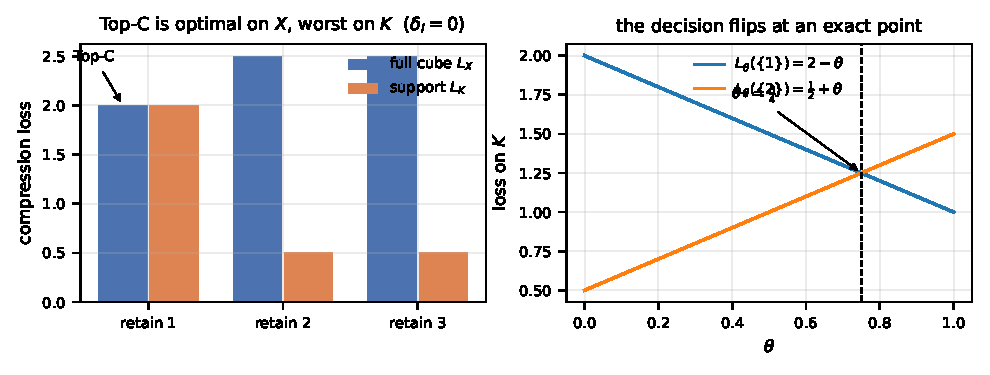
\includegraphics[width=\columnwidth]{unified_support_decision.pdf}
\caption{Left: on the witness of \eqref{eq:witness}, Top-$C$ is optimal on the cube and
worst on the support, with interaction identically zero. Right: along the deformation
\eqref{eq:thetafamily} the decision flips at $\theta_{*}=3/4$.}
\label{fig:support}
\end{figure}

\begin{figure}[t]
\centering
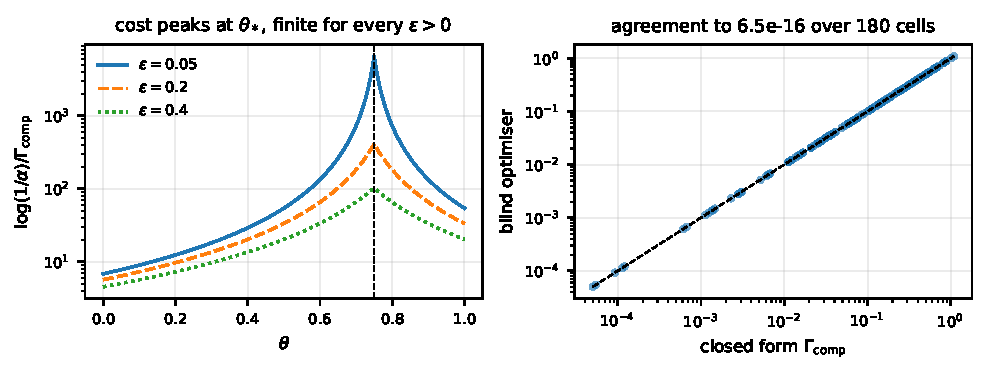
\includegraphics[width=\columnwidth]{unified_calibration.pdf}
\caption{Left: the information-based cost proxy $\log(1/\alpha)/\Gamma_{\rm comp}$, not an
observed or proved stopping cost, peaks at the flip point and
stays finite for every $\varepsilon>0$. Right: a blind optimiser reproduces
\eqref{eq:gamma} at all $180$ cells.}
\label{fig:calibration}
\end{figure}

\begin{figure}[t]
\centering
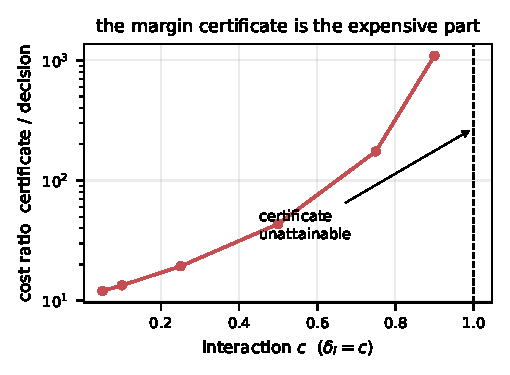
\includegraphics[width=0.78\columnwidth]{unified_oracle_gap.pdf}
\caption{The margin certificate costs orders of magnitude more than the decision it
justifies, and becomes unattainable while the decision stays settled.}
\label{fig:oracle}
\end{figure}

\begin{figure}[t]
\centering
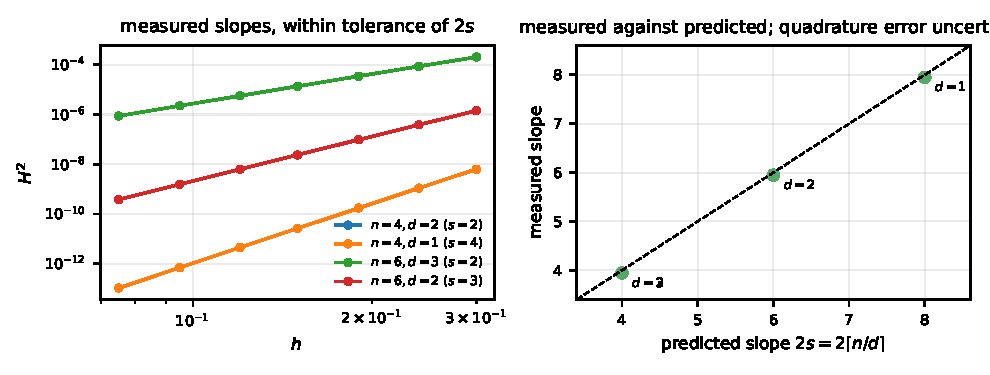
\includegraphics[width=\columnwidth]{unified_query_order.pdf}
\caption{Squared Hellinger distance against $h$, and measured against predicted order.
Exact moments, deterministic quadrature.}
\label{fig:query}
\end{figure}

\begin{figure}[t]
\centering
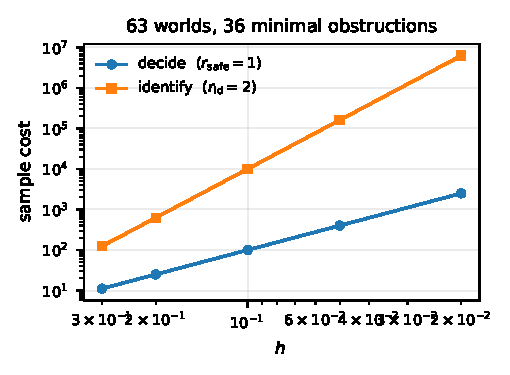
\includegraphics[width=0.78\columnwidth]{unified_obstruction.pdf}
\caption{Illustrative unit-constant exponent proxies for assigned order indices.
These curves are not observed sample counts or a proved complexity separation.}
\label{fig:obstruction}
\end{figure}

\begin{figure}[t]
\centering
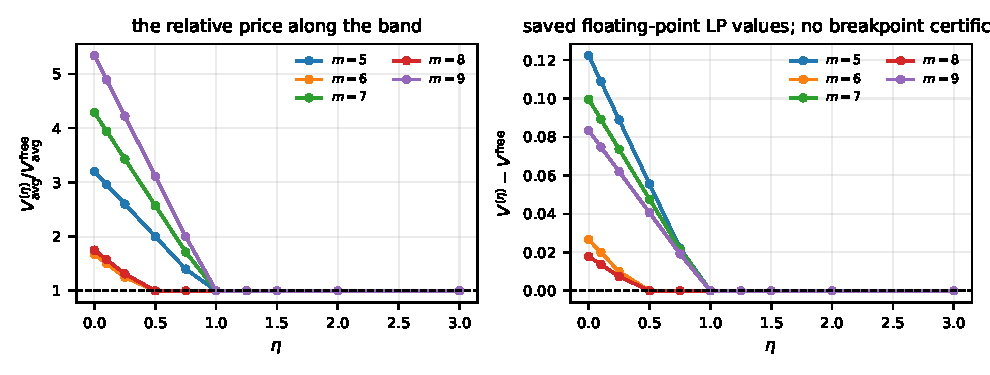
\includegraphics[width=\columnwidth]{unified_structural_frontier.pdf}
\caption{Saved floating-point frontier values. The corrected generator plots the
excess above the free value on the right. The pre-audit PDF instead contains hard-coded
conjectured breakpoints and must be regenerated before submission.}
\label{fig:frontier}
\end{figure}

\section{Limitations}
\label{sec:limits}

We state the boundaries of each claim in the same place as the claim, and collect the
load-bearing ones here.

\begin{enumerate}
\item[1)] \textbf{The geometry rate is computable but not cheaply.}
Theorem~\ref{thm:kappabound} bounds $\kappa$ from $2m$ span values, each requiring certified range access rather than one point or noisy query, and the criterion that
results is vacuous---it fired $0$ times in $919$ trials. The exact constant fires but costs
$\binom{m}{k}$ evaluations, and the $O(m^{2})$ single-swap surrogate is unsound. A
polynomially computable rate strong enough to fire is open.
\item[2)] \textbf{Attainment of the query order is not formalised.} Theorem~\ref{thm:vanish}
proves the vanishing half; the block construction attaining $s!/s^{s}$ is exact arithmetic,
not Lean. Neither adaptive sample-complexity direction follows from vanishing alone.
\item[3)] \textbf{The Gaussian KL is used, not derived.} The profiling and allocation
theorems are statements about a quadratic form; that the form is the weighted KL of the two
location models is standard and assumed.
\item[4)] \textbf{No stopping rule is analysed.} Turning $\Gamma_{\rm comp}$ into
$\log(1/\alpha)/\Gamma_{\rm comp}$ samples needs a geometric tail for this scheme, which we
do not supply.
\item[5)] \textbf{The $\eta$ breakpoints are conjectured, not certified}, and our own bound is not
tight near them.
\item[6)] \textbf{Rates from orders are not formalised.} Section~\ref{sec:obstruction}
supplies the combinatorics and the error floor; converting order-$r$ indistinguishability
into a sample count is the analytic half and is left open.
\item[7)] \textbf{Small configurations throughout.} Three coordinates, two competitors, one
nuisance direction, finitely many worlds and queries. Nothing is claimed about many
components with a changing active alternative set.
\end{enumerate}

\section{Conclusion}

Putting six models into one question produced three quantitative findings and one clean
negative. The support is an independent variable, and the exchange bound needs a geometry
term that a witness shows cannot be dropped. Certifying a margin is strictly, and
sometimes infinitely, more expensive than making the decision it justifies. The obstruction hypergraph suggests a candidate decision-relevant resolution order,
with a randomised error floor that makes a surviving obstruction genuinely costly. And the
constrained-ranking price survives relaxation of the constraint, though the exact
breakpoint remains conjectural. The mechanisms we borrowed are named as
borrowed; what we claim is the specific laws in which these components appear together and
the gaps they produce.

\begin{thebibliography}{00}

\bibitem{degenne2019} R. Degenne and W. M. Koolen, ``Pure exploration with multiple correct
answers,'' in \emph{Advances in Neural Information Processing Systems 32}, 2019,
pp.~14591--14600.

\bibitem{nitinawarat2013} S. Nitinawarat and V. V. Veeravalli, ``Controlled sensing for
sequential multihypothesis testing with controlled Markovian observations and non-uniform
control cost,'' \emph{Sequential Analysis}, vol.~34, no.~1, pp.~1--24, 2015.

\bibitem{grosso2014} V. Grosso, F.-X. Standaert, and E. Prouff, ``Low entropy masking
schemes, revisited,'' in \emph{Smart Card Research and Advanced Applications (CARDIS)},
2013, pp.~33--43.

\bibitem{rioul2021} O. Rioul, W. Cheng, and S. Guilley, ``Cumulant expansion of mutual
information for quantifying leakage of a protected secret,'' in \emph{Proc. IEEE Int. Symp.
Information Theory (ISIT)}, 2021, pp.~2596--2601.

\bibitem{singh2018} A. Singh and T. Joachims, ``Fairness of exposure in rankings,'' in
\emph{Proc. 24th ACM SIGKDD Int. Conf. Knowledge Discovery and Data Mining}, 2018,
pp.~2219--2228.

\bibitem{singh2021} A. Singh, D. Kempe, and T. Joachims, ``Fairness in ranking under
uncertainty,'' in \emph{Advances in Neural Information Processing Systems 34}, 2021,
pp.~11896--11908.

\bibitem{javdani2014} S. Javdani, Y. Chen, A. Karbasi, A. Krause, D. Bagnell, and
S. Srinivasa, ``Near optimal Bayesian active learning for decision making,'' in
\emph{Proc. 17th Int. Conf. Artificial Intelligence and Statistics (AISTATS)}, 2014,
pp.~430--438.

\bibitem{boyd2004} S. Boyd and L. Vandenberghe, \emph{Convex Optimization}. Cambridge,
U.K.: Cambridge Univ. Press, 2004.

\bibitem{pukelsheim2006} F. Pukelsheim, \emph{Optimal Design of Experiments}. Philadelphia,
PA: SIAM Classics in Applied Mathematics, 2006.

\bibitem{odonnell2014} R. O'Donnell, \emph{Analysis of Boolean Functions}. Cambridge,
U.K.: Cambridge Univ. Press, 2014.

\bibitem{mathlib2020} The mathlib Community, ``The Lean mathematical library,'' in
\emph{Proc. 9th ACM SIGPLAN Int. Conf. Certified Programs and Proofs (CPP)}, 2020,
pp.~367--381.

\bibitem{demoura2021} L. de Moura and S. Ullrich, ``The Lean 4 theorem prover and
programming language,'' in \emph{Proc. 28th Int. Conf. Automated Deduction (CADE)}, 2021,
pp.~625--635.

\end{thebibliography}

\appendices
\section{Complete statement inventory}
\label{app:inventory}

The unified-batch development contributes $95$ source-level theorem and lemma declarations across its accepted modules. Those that any step of this paper uses are displayed beside the step that consumes them. This appendix reproduces the \emph{complete} chain---every extracted declaration, grouped by module, including the ones already shown---so that the development can be read end to end without reassembling it from the body.

Each entry is a symbol-level transcription of an extracted Lean source header: Unicode maps to the corresponding \LaTeX{} symbol and identifiers are set upright. The displayed binders and turnstile $\vdash$ follow that source extraction; this is not a guarantee that all elaborated section hypotheses are displayed. The six saved module logs contain 64 explicit axiom prints, not 95 individual
audits. Clean downstream audits cover the declarations they actually depend on, but no
one-to-one audit of all appendix entries is claimed. The source extractor is not a Lean
elaborator or receipt validator; the binder transcription also requires checking against
the elaborated signatures, including section variables.

\vspace{4pt}\noindent\rule{\columnwidth}{0.4pt}\par\vspace{2pt}
\noindent\textbf{Module \lean{LeanUnifiedCompressionDecisionV1}}\par\vspace{3pt}

\noindent\textbf{A\,1}\quad\lean{residt\_p0}
{\footnotesize\[ (\mathit{t} : \mathbb{R} ),\; (\mathit{T} : \mathit{Finset} (\mathit{Fin} 3)) \;\vdash\; \mathit{residt} \mathit{t} \mathit{T} \mathit{p0} = 0 \]}

\noindent\textbf{A\,2}\quad\lean{residt\_first\_p1}
{\footnotesize\[ (\mathit{t} : \mathbb{R} ) \;\vdash\; \mathit{residt} \mathit{t} \{ 0\} \mathit{p1} = -4 + 2 * \mathit{t} \]}

\noindent\textbf{A\,3}\quad\lean{residt\_second\_p1}
{\footnotesize\[ (\mathit{t} : \mathbb{R} ) \;\vdash\; \mathit{residt} \mathit{t} \{ 1\} \mathit{p1} = 1 + 2 * \mathit{t} \]}

\noindent\textbf{A\,4}\quad\lean{mem\_Kw'}
{\footnotesize\[ (\mathit{x} : \mathit{Pt}),\; (\mathit{hx} : \mathit{x} \in \mathit{Kw}) \;\vdash\; \mathit{x} = \mathit{p0} \vee \mathit{x} = \mathit{p1} \]}

\noindent\textbf{A\,5}\quad\lean{loss\_retain\_first}
{\footnotesize\[ \begin{aligned}[t]
&(\mathit{t} : \mathbb{R} ),\; (\mathit{ht} : \mathit{t} \leq 2)\\
\vdash\;&\mathit{lossOn} \mathit{Kw} \mathit{Kw\_nonempty} (\mathit{residt} \mathit{t} \{ 0\} ) = 2 - \mathit{t}
\end{aligned} \]}

\noindent\textbf{A\,6}\quad\lean{loss\_retain\_second}
{\footnotesize\[ \begin{aligned}[t]
&(\mathit{t} : \mathbb{R} ),\; (\mathit{ht} : -1 / 2 \leq \mathit{t})\\
\vdash\;&\mathit{lossOn} \mathit{Kw} \mathit{Kw\_nonempty} (\mathit{residt} \mathit{t} \{ 1\} ) = 1 / 2 + \mathit{t}
\end{aligned} \]}

\noindent\textbf{A\,7}\quad\lean{decision\_flips\_at\_three\_quarters}
{\footnotesize\[ \begin{aligned}[t]
\vdash\;&\mathit{lossOn} \mathit{Kw} \mathit{Kw\_nonempty} (\mathit{residt} (3 / 4) \{ 0\} ) =\\
&\quad \mathit{lossOn} \mathit{Kw} \mathit{Kw\_nonempty} (\mathit{residt} (3 / 4) \{ 1\} )
\end{aligned} \]}

\noindent\textbf{A\,8}\quad\lean{first\_better\_above}
{\footnotesize\[ \begin{aligned}[t]
&(\mathit{t} : \mathbb{R} ),\; (\mathit{h1} : 3 / 4 < \mathit{t}),\; (\mathit{h2} : \mathit{t} \leq 2)\\
\vdash\;&\mathit{lossOn} \mathit{Kw} \mathit{Kw\_nonempty} (\mathit{residt} \mathit{t} \{ 0\} ) < \mathit{lossOn} \mathit{Kw}\\
&\quad \mathit{Kw\_nonempty} (\mathit{residt} \mathit{t} \{ 1\} )
\end{aligned} \]}

\noindent\textbf{A\,9}\quad\lean{second\_better\_below}
{\footnotesize\[ \begin{aligned}[t]
&(\mathit{t} : \mathbb{R} ),\; (\mathit{h1} : -1 / 2 \leq \mathit{t}),\; (\mathit{h2} : \mathit{t} < 3 / 4)\\
\vdash\;&\mathit{lossOn} \mathit{Kw} \mathit{Kw\_nonempty} (\mathit{residt} \mathit{t} \{ 1\} ) < \mathit{lossOn} \mathit{Kw}\\
&\quad \mathit{Kw\_nonempty} (\mathit{residt} \mathit{t} \{ 0\} )
\end{aligned} \]}

\noindent\textbf{A\,10}\quad\lean{safe\_first\_iff}
{\footnotesize\[ \begin{aligned}[t]
&(\mathit{t} \mathit{eps} : \mathbb{R} ),\; (\mathit{heps} : 0 \leq \mathit{eps})\\
\vdash\;&(2 - \mathit{t}) - \mathit{min} (2 - \mathit{t}) (1 / 2 + \mathit{t}) \leq \mathit{eps} \leftrightarrow 3 / 4 - \mathit{eps} / 2 \leq \mathit{t}
\end{aligned} \]}

\noindent\textbf{A\,11}\quad\lean{safe\_second\_iff}
{\footnotesize\[ \begin{aligned}[t]
&(\mathit{t} \mathit{eps} : \mathbb{R} ),\; (\mathit{heps} : 0 \leq \mathit{eps})\\
\vdash\;&(1 / 2 + \mathit{t}) - \mathit{min} (2 - \mathit{t}) (1 / 2 + \mathit{t}) \leq \mathit{eps} \leftrightarrow \mathit{t} \leq\\
&\quad 3 / 4 + \mathit{eps} / 2
\end{aligned} \]}

\noindent\textbf{A\,12}\quad\lean{decision\_distance\_eq}
{\footnotesize\[ \begin{aligned}[t]
&(\mathit{t} \mathit{eps} : \mathbb{R} )\\
\vdash\;&(\mathbf{if} 3 / 4 \leq \mathit{t} \mathbf{then} \mathit{t} - (3 / 4 - \mathit{eps} / 2) \mathbf{else} (3 / 4 + \mathit{eps} / 2) -\\
&\quad \mathit{t}) = |\mathit{t} - 3 / 4| + \mathit{eps} / 2
\end{aligned} \]}

\noindent\textbf{A\,13}\quad\lean{nuisance\_profiled\_information}
{\footnotesize\[ \begin{aligned}[t]
&(\mathit{wo} \mathit{wa} \mathit{sigma} \mathit{nu} \mathit{D} \mathit{u} : \mathbb{R} ),\; (\mathit{hwo} : 0 < \mathit{wo}),\; (\mathit{hwa} : 0 < \mathit{wa}),\\
&\quad \; (\mathit{hs} : 0 < \mathit{sigma}),\; (\mathit{hn} : 0 < \mathit{nu})\\
\vdash\;&\mathit{D} ^{2} / (2 * (\mathit{sigma} ^{2} / \mathit{wo} + \mathit{nu} ^{2} / \mathit{wa})) \leq \mathit{wo} * (\mathit{D} + \mathit{u}) ^{2} / (2 *\\
&\quad \mathit{sigma} ^{2}) + \mathit{wa} * \mathit{u} ^{2} / (2 * \mathit{nu} ^{2})
\end{aligned} \]}

\noindent\textbf{A\,14}\quad\lean{allocation\_lower\_bound}
{\footnotesize\[ \begin{aligned}[t]
&(\mathit{wo} \mathit{wa} \mathit{sigma} \mathit{nu} \mathit{s} \mathit{r} : \mathbb{R} ),\; (\mathit{hwo} : 0 < \mathit{wo}),\; (\mathit{hwa} : 0 < \mathit{wa}),\\
&\quad \; (\mathit{hs} : 0 < \mathit{s}),\; (\mathit{hr} : 0 < \mathit{r}),\; (\mathit{hsig} : 0 < \mathit{sigma}),\\
&\quad \; (\mathit{hnu} : 0 < \mathit{nu}),\; (\mathit{hbudget} : \mathit{s} ^{2} * \mathit{wo} + \mathit{r} ^{2} * \mathit{wa} = 1)\\
\vdash\;&(\mathit{sigma} * \mathit{s} + \mathit{nu} * \mathit{r}) ^{2} \leq \mathit{sigma} ^{2} / \mathit{wo} + \mathit{nu} ^{2} / \mathit{wa}
\end{aligned} \]}

\noindent\textbf{A\,15}\quad\lean{allocation\_optimum\_attained}
{\footnotesize\[ \begin{aligned}[t]
&(\mathit{sigma} \mathit{nu} \mathit{s} \mathit{r} : \mathbb{R} ),\; (\mathit{hs} : 0 < \mathit{s}),\; (\mathit{hr} : 0 < \mathit{r}),\\
&\quad \; (\mathit{hsig} : 0 < \mathit{sigma}),\; (\mathit{hnu} : 0 < \mathit{nu})\\
\vdash\;&\mathit{s} ^{2} * (\mathit{sigma} / (\mathit{s} * (\mathit{sigma} * \mathit{s} + \mathit{nu} * \mathit{r}))) + \mathit{r} ^{2} * (\mathit{nu} / (\mathit{r} * (\\
&\quad \mathit{sigma} * \mathit{s} + \mathit{nu} * \mathit{r}))) = 1 \wedge \mathit{sigma} ^{2} / (\mathit{sigma} / (\mathit{s} * (\mathit{sigma} *\\
&\quad \mathit{s} + \mathit{nu} * \mathit{r}))) + \mathit{nu} ^{2} / (\mathit{nu} / (\mathit{r} * (\mathit{sigma} * \mathit{s} + \mathit{nu} * \mathit{r}))) =\\
&\quad (\mathit{sigma} * \mathit{s} + \mathit{nu} * \mathit{r}) ^{2}
\end{aligned} \]}

\noindent\textbf{A\,16}\quad\lean{gamma\_comp\_eq}
{\footnotesize\[ \begin{aligned}[t]
&(\mathit{Delta} \mathit{sigma} \mathit{nu} \mathit{s} \mathit{r} : \mathbb{R} ),\; (\mathit{hs} : 0 < \mathit{s}),\; (\mathit{hr} : 0 < \mathit{r}),\\
&\quad \; (\mathit{hsig} : 0 < \mathit{sigma}),\; (\mathit{hnu} : 0 < \mathit{nu})\\
\vdash\;&(3 * \mathit{Delta}) ^{2} / (2 * (\mathit{sigma} * \mathit{s} + \mathit{nu} * \mathit{r}) ^{2}) =\\
&\quad 9 * \mathit{Delta} ^{2} / (2 * (\mathit{sigma} * \mathit{s} + \mathit{nu} * \mathit{r}) ^{2})
\end{aligned} \]}

\noindent\textbf{A\,17}\quad\lean{game\_value\_upper}
{\footnotesize\[ \begin{aligned}[t]
&(\mathit{wo} \mathit{wa} \mathit{sigma} \mathit{nu} \mathit{s} \mathit{r} \mathit{Delta} : \mathbb{R} ),\; (\mathit{hwo} : 0 < \mathit{wo}),\; (\mathit{hwa} : 0 < \mathit{wa}),\\
&\quad \; (\mathit{hs} : 0 < \mathit{s}),\; (\mathit{hr} : 0 < \mathit{r}),\; (\mathit{hsig} : 0 < \mathit{sigma}),\\
&\quad \; (\mathit{hnu} : 0 < \mathit{nu}),\; (\mathit{hbudget} : \mathit{s} ^{2} * \mathit{wo} + \mathit{r} ^{2} * \mathit{wa} = 1)\\
\vdash\;&(3 * \mathit{Delta}) ^{2} / (2 * (\mathit{sigma} ^{2} / \mathit{wo} + \mathit{nu} ^{2} / \mathit{wa})) \leq\\
&\quad (3 * \mathit{Delta}) ^{2} / (2 * (\mathit{sigma} * \mathit{s} + \mathit{nu} * \mathit{r}) ^{2})
\end{aligned} \]}

\noindent\textbf{A\,18}\quad\lean{confounded\_pair\_same\_law}
{\footnotesize\[ \vdash\; \mathit{meanY} 0 0 = \mathit{meanY} 1 (-3) \]}

\noindent\textbf{A\,19}\quad\lean{confounded\_pair\_need\_different\_answers}
{\footnotesize\[ \begin{aligned}[t]
&(\mathit{eps} : \mathbb{R} ),\; (\mathit{heps} : 0 \leq \mathit{eps}),\; (\mathit{hlt} : \mathit{eps} < 1 / 2)\\
\vdash\;&\neg ((2 - (0:\mathbb{R} )) - \mathit{min} (2 - (0:\mathbb{R} )) (1 / 2 + (0:\mathbb{R} )) \leq \mathit{eps}) \wedge\\
&\quad \neg ((1 / 2 + (1:\mathbb{R} )) - \mathit{min} (2 - (1:\mathbb{R} )) (1 / 2 + (1:\mathbb{R} )) \leq \mathit{eps})
\end{aligned} \]}

\noindent\textbf{A\,20}\quad\lean{no\_measurement\_phase}
{\footnotesize\[ \begin{aligned}[t]
&(\mathit{t} \mathit{eps} : \mathbb{R} ),\; (\mathit{h0} : 0 \leq \mathit{t}),\; (\mathit{h1} : \mathit{t} \leq 1),\; (\mathit{heps} : 1 / 2 \leq \mathit{eps})\\
\vdash\;&(1 / 2 + \mathit{t}) - \mathit{min} (2 - \mathit{t}) (1 / 2 + \mathit{t}) \leq \mathit{eps}
\end{aligned} \]}

\vspace{4pt}\noindent\rule{\columnwidth}{0.4pt}\par\vspace{2pt}
\noindent\textbf{Module \lean{LeanUnifiedGeometryBoundV1}}\par\vspace{3pt}

\noindent\textbf{A\,21}\quad\lean{le\_maxOn}
{\footnotesize\[ \begin{aligned}[t]
&(\mathit{S} : \mathit{Finset} \mathit{A}),\; (\mathit{hS} : \mathit{S}.\mathit{Nonempty}),\; (\mathit{f} : \mathit{A} \to \mathbb{R} ),\\
&\quad \; \{ \mathit{a} : \mathit{A}\},\; (\mathit{ha} : \mathit{a} \in \mathit{S})\\
\vdash\;&\mathit{f} \mathit{a} \leq \mathit{maxOn} \mathit{S} \mathit{hS} \mathit{f}
\end{aligned} \]}

\noindent\textbf{A\,22}\quad\lean{minOn\_le}
{\footnotesize\[ \begin{aligned}[t]
&(\mathit{S} : \mathit{Finset} \mathit{A}),\; (\mathit{hS} : \mathit{S}.\mathit{Nonempty}),\; (\mathit{f} : \mathit{A} \to \mathbb{R} ),\\
&\quad \; \{ \mathit{a} : \mathit{A}\},\; (\mathit{ha} : \mathit{a} \in \mathit{S})\\
\vdash\;&\mathit{minOn} \mathit{S} \mathit{hS} \mathit{f} \leq \mathit{f} \mathit{a}
\end{aligned} \]}

\noindent\textbf{A\,23}\quad\lean{maxOn\_le\_of}
{\footnotesize\[ \begin{aligned}[t]
&(\mathit{S} : \mathit{Finset} \mathit{A}),\; (\mathit{hS} : \mathit{S}.\mathit{Nonempty}),\; (\mathit{f} : \mathit{A} \to \mathbb{R} ),\; (\mathit{b} : \mathbb{R} ),\\
&\quad \; (\mathit{h} : \forall \mathit{x} \in \mathit{S}, \mathit{f} \mathit{x} \leq \mathit{b})\\
\vdash\;&\mathit{maxOn} \mathit{S} \mathit{hS} \mathit{f} \leq \mathit{b}
\end{aligned} \]}

\noindent\textbf{A\,24}\quad\lean{le\_minOn\_of}
{\footnotesize\[ \begin{aligned}[t]
&(\mathit{S} : \mathit{Finset} \mathit{A}),\; (\mathit{hS} : \mathit{S}.\mathit{Nonempty}),\; (\mathit{f} : \mathit{A} \to \mathbb{R} ),\; (\mathit{b} : \mathbb{R} ),\\
&\quad \; (\mathit{h} : \forall \mathit{x} \in \mathit{S}, \mathit{b} \leq \mathit{f} \mathit{x})\\
\vdash\;&\mathit{b} \leq \mathit{minOn} \mathit{S} \mathit{hS} \mathit{f}
\end{aligned} \]}

\noindent\textbf{A\,25}\quad\lean{exists\_maxOn}
{\footnotesize\[ \begin{aligned}[t]
&(\mathit{S} : \mathit{Finset} \mathit{A}),\; (\mathit{hS} : \mathit{S}.\mathit{Nonempty}),\; (\mathit{f} : \mathit{A} \to \mathbb{R} )\\
\vdash\;&\exists \mathit{a} \in \mathit{S}, \mathit{f} \mathit{a} = \mathit{maxOn} \mathit{S} \mathit{hS} \mathit{f}
\end{aligned} \]}

\noindent\textbf{A\,26}\quad\lean{exists\_minOn}
{\footnotesize\[ \begin{aligned}[t]
&(\mathit{S} : \mathit{Finset} \mathit{A}),\; (\mathit{hS} : \mathit{S}.\mathit{Nonempty}),\; (\mathit{f} : \mathit{A} \to \mathbb{R} )\\
\vdash\;&\exists \mathit{a} \in \mathit{S}, \mathit{f} \mathit{a} = \mathit{minOn} \mathit{S} \mathit{hS} \mathit{f}
\end{aligned} \]}

\noindent\textbf{A\,27}\quad\lean{oscOn\_nonneg}
{\footnotesize\[ \begin{aligned}[t]
&(\mathit{S} : \mathit{Finset} \mathit{A}),\; (\mathit{hS} : \mathit{S}.\mathit{Nonempty}),\; (\mathit{f} : \mathit{A} \to \mathbb{R} )\\
\vdash\;&0 \leq \mathit{oscOn} \mathit{S} \mathit{hS} \mathit{f}
\end{aligned} \]}

\noindent\textbf{A\,28}\quad\lean{oscOn\_const}
{\footnotesize\[ \begin{aligned}[t]
&(\mathit{S} : \mathit{Finset} \mathit{A}),\; (\mathit{hS} : \mathit{S}.\mathit{Nonempty}),\; (\mathit{b} : \mathbb{R} )\\
\vdash\;&\mathit{oscOn} \mathit{S} \mathit{hS} (\mathbf{fun} \mathit{\_} => \mathit{b}) = 0
\end{aligned} \]}

\noindent\textbf{A\,29}\quad\lean{oscOn\_add\_le}
{\footnotesize\[ \begin{aligned}[t]
&(\mathit{S} : \mathit{Finset} \mathit{A}),\; (\mathit{hS} : \mathit{S}.\mathit{Nonempty}),\; (\mathit{f} \mathit{g} : \mathit{A} \to \mathbb{R} )\\
\vdash\;&\mathit{oscOn} \mathit{S} \mathit{hS} (\mathbf{fun} \mathit{x} => \mathit{f} \mathit{x} + \mathit{g} \mathit{x}) \leq \mathit{oscOn} \mathit{S} \mathit{hS} \mathit{f} + \mathit{oscOn} \mathit{S} \mathit{hS} \mathit{g}
\end{aligned} \]}

\noindent\textbf{A\,30}\quad\lean{oscOn\_neg}
{\footnotesize\[ \begin{aligned}[t]
&(\mathit{S} : \mathit{Finset} \mathit{A}),\; (\mathit{hS} : \mathit{S}.\mathit{Nonempty}),\; (\mathit{f} : \mathit{A} \to \mathbb{R} )\\
\vdash\;&\mathit{oscOn} \mathit{S} \mathit{hS} (\mathbf{fun} \mathit{x} => -\mathit{f} \mathit{x}) = \mathit{oscOn} \mathit{S} \mathit{hS} \mathit{f}
\end{aligned} \]}

\noindent\textbf{A\,31}\quad\lean{oscOn\_sub\_le}
{\footnotesize\[ \begin{aligned}[t]
&(\mathit{S} : \mathit{Finset} \mathit{A}),\; (\mathit{hS} : \mathit{S}.\mathit{Nonempty}),\; (\mathit{f} \mathit{g} : \mathit{A} \to \mathbb{R} )\\
\vdash\;&\mathit{oscOn} \mathit{S} \mathit{hS} (\mathbf{fun} \mathit{x} => \mathit{f} \mathit{x} - \mathit{g} \mathit{x}) \leq \mathit{oscOn} \mathit{S} \mathit{hS} \mathit{f} + \mathit{oscOn} \mathit{S} \mathit{hS} \mathit{g}
\end{aligned} \]}

\noindent\textbf{A\,32}\quad\lean{oscOn\_sum\_le}
{\footnotesize\[ \begin{aligned}[t]
&\{ \iota : \mathit{Type}*\},\; [\mathit{DecidableEq} \iota ],\; (\mathit{S} : \mathit{Finset} \mathit{A}),\; (\mathit{hS} : \mathit{S}.\mathit{Nonempty})\\
&\quad ,\; (\mathit{Q} : \iota \to \mathit{A} \to \mathbb{R} ),\; (\mathit{E} : \mathit{Finset} \iota )\\
\vdash\;&\mathit{oscOn} \mathit{S} \mathit{hS} (\mathbf{fun} \mathit{x} => \textstyle\sum \mathit{j} \in \mathit{E}, \mathit{Q} \mathit{j} \mathit{x}) \leq \textstyle\sum \mathit{j} \in \mathit{E}, \mathit{oscOn} \mathit{S} \mathit{hS} (\mathit{Q} \mathit{j})
\end{aligned} \]}

\noindent\textbf{A\,33}\quad\lean{geomGap\_eq\_of\_modular}
{\footnotesize\[ \begin{aligned}[t]
&(\mathit{K} \mathit{X} : \mathit{Finset} \mathit{A}),\; (\mathit{hK} : \mathit{K}.\mathit{Nonempty}),\; (\mathit{hX} : \mathit{X}.\\
&\quad \mathit{Nonempty}),\; (\mathit{Q} : \iota \to \mathit{A} \to \mathbb{R} ),\; (\mathit{E} : \mathit{Finset} \iota ),\\
&\quad \; (\mathit{hmod} : \mathit{oscOn} \mathit{X} \mathit{hX} (\mathit{sumOver} \mathit{Q} \mathit{E}) = \textstyle\sum \mathit{j} \in \mathit{E}, \mathit{oscOn} \mathit{X} \mathit{hX} (\mathit{Q}\\
&\quad \mathit{j}))\\
\vdash\;&\mathit{geomGap} \mathit{K} \mathit{X} \mathit{hK} \mathit{hX} (\mathit{sumOver} \mathit{Q} \mathit{E}) = ((\textstyle\sum \mathit{j} \in \mathit{E}, \mathit{oscOn} \mathit{X} \mathit{hX} (\mathit{Q}\\
&\quad \mathit{j})) - \mathit{oscOn} \mathit{K} \mathit{hK} (\mathit{sumOver} \mathit{Q} \mathit{E})) / 2
\end{aligned} \]}

\noindent\textbf{A\,34}\quad\lean{compl\_sdiff\_compl}
{\footnotesize\[ (\mathit{S} \mathit{T} : \mathit{Finset} \iota ) \;\vdash\; \mathit{Sᶜ} \ \mathit{Tᶜ} = \mathit{T} \ \mathit{S} \]}

\noindent\textbf{A\,35}\quad\lean{geomGap\_diff\_le\_spans}
{\footnotesize\[ \begin{aligned}[t]
&(\mathit{K} \mathit{X} : \mathit{Finset} \mathit{A}),\; (\mathit{hK} : \mathit{K}.\mathit{Nonempty}),\; (\mathit{hX} : \mathit{X}.\\
&\quad \mathit{Nonempty}),\; (\mathit{hsub} : \mathit{K} \subseteq \mathit{X}),\; (\mathit{Q} : \iota \to \mathit{A} \to \mathbb{R} ),\\
&\quad \; (\mathit{T} \mathit{S} : \mathit{Finset} \iota ),\; (\mathit{hmod} : \forall \mathit{E} : \mathit{Finset} \iota , \mathit{oscOn} \mathit{X} \mathit{hX} (\\
&\quad \mathit{sumOver} \mathit{Q} \mathit{E}) = \textstyle\sum \mathit{j} \in \mathit{E}, \mathit{oscOn} \mathit{X} \mathit{hX} (\mathit{Q} \mathit{j}))\\
\vdash\;&\mathit{geomGap} \mathit{K} \mathit{X} \mathit{hK} \mathit{hX} (\mathit{sumOver} \mathit{Q} \mathit{Sᶜ}) - \mathit{geomGap} \mathit{K} \mathit{X} \mathit{hK} \mathit{hX} (\\
&\quad \mathit{sumOver} \mathit{Q} \mathit{Tᶜ}) \leq (\textstyle\sum \mathit{j} \in \mathit{T} \ \mathit{S}, (\mathit{oscOn} \mathit{X} \mathit{hX} (\mathit{Q} \mathit{j}) + \mathit{oscOn} \mathit{K} \mathit{hK}\\
&\quad (\mathit{Q} \mathit{j}))) / 2
\end{aligned} \]}

\noindent\textbf{A\,36}\quad\lean{kappa\_of\_spans}
{\footnotesize\[ \begin{aligned}[t]
&(\mathit{K} \mathit{X} : \mathit{Finset} \mathit{A}),\; (\mathit{hK} : \mathit{K}.\mathit{Nonempty}),\; (\mathit{hX} : \mathit{X}.\\
&\quad \mathit{Nonempty}),\; (\mathit{hsub} : \mathit{K} \subseteq \mathit{X}),\; (\mathit{Q} : \iota \to \mathit{A} \to \mathbb{R} ),\\
&\quad \; (\mathit{T} \mathit{S} : \mathit{Finset} \iota ),\; (\mathit{kappa} : \mathbb{R} ),\; (\mathit{hmod} : \forall \mathit{E} : \mathit{Finset} \iota\\
&\quad , \mathit{oscOn} \mathit{X} \mathit{hX} (\mathit{sumOver} \mathit{Q} \mathit{E}) = \textstyle\sum \mathit{j} \in \mathit{E}, \mathit{oscOn} \mathit{X} \mathit{hX} (\mathit{Q} \mathit{j})),\\
&\quad \; (\mathit{hkap} : \forall \mathit{j} \in \mathit{T}, (\mathit{oscOn} \mathit{X} \mathit{hX} (\mathit{Q} \mathit{j}) + \mathit{oscOn} \mathit{K} \mathit{hK} (\mathit{Q} \mathit{j})) /\\
&\quad 2 \leq \mathit{kappa})\\
\vdash\;&\mathit{geomGap} \mathit{K} \mathit{X} \mathit{hK} \mathit{hX} (\mathit{sumOver} \mathit{Q} \mathit{Sᶜ}) - \mathit{geomGap} \mathit{K} \mathit{X} \mathit{hK} \mathit{hX} (\\
&\quad \mathit{sumOver} \mathit{Q} \mathit{Tᶜ}) \leq \mathit{kappa} * ((\mathit{T} \ \mathit{S}).\mathit{card} : \mathbb{R} )
\end{aligned} \]}

\noindent\textbf{A\,37}\quad\lean{computable\_threshold}
{\footnotesize\[ \begin{aligned}[t]
&(\mathit{K} \mathit{X} : \mathit{Finset} \mathit{A}),\; (\mathit{hK} : \mathit{K}.\mathit{Nonempty}),\; (\mathit{hX} : \mathit{X}.\mathit{Nonempty}),\\
&\quad \; (\mathit{hsub} : \mathit{K} \subseteq \mathit{X}),\; (\mathit{Q} : \iota \to \mathit{A} \to \mathbb{R} ),\; (\mathit{T} \mathit{S} : \mathit{Finset} \iota ),\\
&\quad \; (\mathit{delta} \mathit{rho} \mathit{kappa} : \mathbb{R} ),\; (\mathit{hmod} : \forall \mathit{E} : \mathit{Finset} \iota , \mathit{oscOn} \mathit{X} \mathit{hX} (\\
&\quad \mathit{sumOver} \mathit{Q} \mathit{E}) = \textstyle\sum \mathit{j} \in \mathit{E}, \mathit{oscOn} \mathit{X} \mathit{hX} (\mathit{Q} \mathit{j})),\; (\mathit{hkap} : \forall \mathit{j} \in \mathit{T},\\
&\quad (\mathit{oscOn} \mathit{X} \mathit{hX} (\mathit{Q} \mathit{j}) + \mathit{oscOn} \mathit{K} \mathit{hK} (\mathit{Q} \mathit{j})) / 2 \leq \mathit{kappa}),\\
&\quad \; (\mathit{hfull} : 2 * (\mathit{lossOn} \mathit{X} \mathit{hX} (\mathit{sumOver} \mathit{Q} \mathit{Tᶜ}) - \mathit{lossOn} \mathit{X} \mathit{hX} (\\
&\quad \mathit{sumOver} \mathit{Q} \mathit{Sᶜ})) \leq (((\mathit{T} \ \mathit{S}).\mathit{card} : \mathbb{N} ) : \mathbb{R} ) * (2 * \mathit{delta} -\\
&\quad \mathit{rho})),\; (\mathit{hthr} : 2 * \mathit{delta} + 2 * \mathit{kappa} \leq \mathit{rho})\\
\vdash\;&\mathit{lossOn} \mathit{K} \mathit{hK} (\mathit{sumOver} \mathit{Q} \mathit{Tᶜ}) \leq \mathit{lossOn} \mathit{K} \mathit{hK} (\mathit{sumOver} \mathit{Q} \mathit{Sᶜ})
\end{aligned} \]}

\vspace{4pt}\noindent\rule{\columnwidth}{0.4pt}\par\vspace{2pt}
\noindent\textbf{Module \lean{LeanUnifiedObstructionOrderV1}}\par\vspace{3pt}

\noindent\textbf{A\,38}\quad\lean{hasCommon\_mono}
{\footnotesize\[ \begin{aligned}[t]
&\{ \mathit{H} \mathit{H'} : \mathit{Finset} \mathit{World}\},\; (\mathit{hsub} : \mathit{H} \subseteq \mathit{H'}),\; (\mathit{h} : \mathit{HasCommon} \mathit{safe}\\
&\quad \mathit{H'})\\
\vdash\;&\mathit{HasCommon} \mathit{safe} \mathit{H}
\end{aligned} \]}

\noindent\textbf{A\,39}\quad\lean{isObstruction\_mono}
{\footnotesize\[ \begin{aligned}[t]
&\{ \mathit{H} \mathit{H'} : \mathit{Finset} \mathit{World}\},\; (\mathit{hsub} : \mathit{H} \subseteq \mathit{H'}),\; (\mathit{h} : \mathit{IsObstruction} \mathit{safe}\\
&\quad \mathit{H})\\
\vdash\;&\mathit{IsObstruction} \mathit{safe} \mathit{H'}
\end{aligned} \]}

\noindent\textbf{A\,40}\quad\lean{classes\_resolve\_iff}
{\footnotesize\[ \begin{aligned}[t]
&\{ \mathit{K} : \mathit{Type}*\},\; [\mathit{DecidableEq} \mathit{K}],\; [\mathit{Fintype} \mathit{K}],\\
&\quad \; (\mathit{cls} : \mathit{World} \to \mathit{K})\\
\vdash\;&(\forall \mathit{k} : \mathit{K}, \mathit{HasCommon} \mathit{safe} (\mathit{univ}.\mathit{filter} (\mathbf{fun} \mathit{F} => \mathit{cls} \mathit{F} = \mathit{k}))\\
&\quad ) \leftrightarrow (\forall \mathit{H} : \mathit{Finset} \mathit{World}, \mathit{IsObstruction} \mathit{safe} \mathit{H} \to \neg \exists \mathit{k} : \mathit{K},\\
&\quad \mathit{H} \subseteq \mathit{univ}.\mathit{filter} (\mathbf{fun} \mathit{F} => \mathit{cls} \mathit{F} = \mathit{k}))
\end{aligned} \]}

\noindent\textbf{A\,41}\quad\lean{resolution\_refines}
{\footnotesize\[ \begin{aligned}[t]
&[\mathit{Nonempty} \mathit{Act}],\; \{ \mathit{K} \mathit{L} : \mathit{Type}*\},\; [\mathit{DecidableEq} \mathit{K}],\\
&\quad \; [\mathit{DecidableEq} \mathit{L}],\; [\mathit{Fintype} \mathit{K}],\; [\mathit{Fintype} \mathit{L}],\; (\mathit{coarse} : \mathit{World}\\
&\quad \to \mathit{K}),\; (\mathit{fine} : \mathit{World} \to \mathit{L}),\; (\mathit{hrefine} : \forall \mathit{F} \mathit{G} : \mathit{World}, \mathit{fine} \mathit{F} =\\
&\quad \mathit{fine} \mathit{G} \to \mathit{coarse} \mathit{F} = \mathit{coarse} \mathit{G}),\; (\mathit{hcoarse} : \forall \mathit{k} : \mathit{K},\\
&\quad \mathit{HasCommon} \mathit{safe} (\mathit{univ}.\mathit{filter} (\mathbf{fun} \mathit{F} => \mathit{coarse} \mathit{F} = \mathit{k})))\\
\vdash\;&\forall \mathit{l} : \mathit{L}, \mathit{HasCommon} \mathit{safe} (\mathit{univ}.\mathit{filter} (\mathbf{fun} \mathit{F} => \mathit{fine} \mathit{F} = \mathit{l}))
\end{aligned} \]}

\noindent\textbf{A\,42}\quad\lean{obstruction\_error\_floor\_deterministic}
{\footnotesize\[ \begin{aligned}[t]
&\{ \mathit{H} : \mathit{Finset} \mathit{World}\},\; (\mathit{hH} : \mathit{IsObstruction} \mathit{safe} \mathit{H}),\; (\mathit{a} : \mathit{Act})\\
\vdash\;&\exists \mathit{F} \in \mathit{H}, \mathit{a} \notin \mathit{safe} \mathit{F}
\end{aligned} \]}

\noindent\textbf{A\,43}\quad\lean{obstruction\_total\_unsafe\_mass}
{\footnotesize\[ \begin{aligned}[t]
&\{ \mathit{H} : \mathit{Finset} \mathit{World}\},\; (\mathit{hH} : \mathit{IsObstruction} \mathit{safe} \mathit{H}),\; (\mathit{p} : \mathit{Act} \to \mathbb{R} ),\\
&\quad \; (\mathit{hp} : \forall \mathit{a}, 0 \leq \mathit{p} \mathit{a}),\; (\mathit{hsum} : \textstyle\sum \mathit{a}, \mathit{p} \mathit{a} = 1)\\
\vdash\;&1 \leq \textstyle\sum \mathit{F} \in \mathit{H}, \mathit{unsafeMass} \mathit{safe} \mathit{p} \mathit{F}
\end{aligned} \]}

\noindent\textbf{A\,44}\quad\lean{obstruction\_error\_floor\_randomized}
{\footnotesize\[ \begin{aligned}[t]
&\{ \mathit{H} : \mathit{Finset} \mathit{World}\},\; (\mathit{hH} : \mathit{IsObstruction} \mathit{safe} \mathit{H}),\; (\mathit{hne} : \mathit{H}.\\
&\quad \mathit{Nonempty}),\; (\mathit{p} : \mathit{Act} \to \mathbb{R} ),\; (\mathit{hp} : \forall \mathit{a}, 0 \leq \mathit{p} \mathit{a}),\; (\mathit{hsum} : \textstyle\sum \mathit{a},\\
&\quad \mathit{p} \mathit{a} = 1)\\
\vdash\;&\exists \mathit{F} \in \mathit{H}, 1 / (\mathit{H}.\mathit{card} : \mathbb{R} ) \leq \mathit{unsafeMass} \mathit{safe} \mathit{p} \mathit{F}
\end{aligned} \]}

\noindent\textbf{A\,45}\quad\lean{no\_obstruction\_iff\_global\_answer}
{\footnotesize\[ \begin{aligned}[t]
\vdash\;&\mathit{HasCommon} \mathit{safe} (\mathit{univ} : \mathit{Finset} \mathit{World}) \leftrightarrow \forall \mathit{H} : \mathit{Finset} \mathit{World},\\
&\quad \neg \mathit{IsObstruction} \mathit{safe} \mathit{H}
\end{aligned} \]}

\vspace{4pt}\noindent\rule{\columnwidth}{0.4pt}\par\vspace{2pt}
\noindent\textbf{Module \lean{LeanUnifiedQueryOrderV1}}\par\vspace{3pt}

\noindent\textbf{A\,46}\quad\lean{chiS\_mul}
{\footnotesize\[ \begin{aligned}[t]
&(\mathit{S} \mathit{T} : \mathit{Finset} (\mathit{Fin} \mathit{n})),\; (\mathit{z} : \mathit{Fin} \mathit{n} \to \mathit{Bool})\\
\vdash\;&\mathit{chiS} \mathit{S} \mathit{z} * \mathit{chiS} \mathit{T} \mathit{z} = \mathit{chiS} (\mathit{symmDiff} \mathit{S} \mathit{T}) \mathit{z}
\end{aligned} \]}

\noindent\textbf{A\,47}\quad\lean{expect\_chi}
{\footnotesize\[ \begin{aligned}[t]
&(\mathit{S} : \mathit{Finset} (\mathit{Fin} \mathit{n}))\\
\vdash\;&\textstyle\sum \mathit{z} : \mathit{Fin} \mathit{n} \to \mathit{Bool}, \mathit{chiS} \mathit{S} \mathit{z} = \mathbf{if} \mathit{S} = \emptyset \mathbf{then} (2 : \mathbb{R} ) ^{\mathit{n}} \mathbf{else} 0
\end{aligned} \]}

\noindent\textbf{A\,48}\quad\lean{HasDeg\_one}
{\footnotesize\[ \vdash\; \mathit{HasDeg} (\mathit{n} := \mathit{n}) 0 (\mathbf{fun} \mathit{\_} => 1) \]}

\noindent\textbf{A\,49}\quad\lean{HasDeg\_mono}
{\footnotesize\[ \begin{aligned}[t]
&\{ \mathit{D} \mathit{D'} : \mathbb{N} \},\; \{ \mathit{h} : (\mathit{Fin} \mathit{n} \to \mathit{Bool}) \to \mathbb{R} \},\; (\mathit{hD} : \mathit{D} \leq \mathit{D'}),\\
&\quad \; (\mathit{hh} : \mathit{HasDeg} \mathit{D} \mathit{h})\\
\vdash\;&\mathit{HasDeg} \mathit{D'} \mathit{h}
\end{aligned} \]}

\noindent\textbf{A\,50}\quad\lean{card\_symmDiff\_le}
{\footnotesize\[ (\mathit{S} \mathit{T} : \mathit{Finset} (\mathit{Fin} \mathit{n})) \;\vdash\; (\mathit{symmDiff} \mathit{S} \mathit{T}).\mathit{card} \leq \mathit{S}.\mathit{card} + \mathit{T}.\mathit{card} \]}

\noindent\textbf{A\,51}\quad\lean{HasDeg\_mul}
{\footnotesize\[ \begin{aligned}[t]
&\{ \mathit{D₁} \mathit{D₂} : \mathbb{N} \},\; \{ \mathit{h₁} \mathit{h₂} : (\mathit{Fin} \mathit{n} \to \mathit{Bool}) \to \mathbb{R} \},\; (\mathit{hh₁} : \mathit{HasDeg} \mathit{D₁} \mathit{h₁}),\\
&\quad \; (\mathit{hh₂} : \mathit{HasDeg} \mathit{D₂} \mathit{h₂})\\
\vdash\;&\mathit{HasDeg} (\mathit{D₁} + \mathit{D₂}) (\mathbf{fun} \mathit{z} => \mathit{h₁} \mathit{z} * \mathit{h₂} \mathit{z})
\end{aligned} \]}

\noindent\textbf{A\,52}\quad\lean{HasDeg\_pow}
{\footnotesize\[ \begin{aligned}[t]
&\{ \mathit{D} : \mathbb{N} \},\; \{ \mathit{h} : (\mathit{Fin} \mathit{n} \to \mathit{Bool}) \to \mathbb{R} \},\; (\mathit{hh} : \mathit{HasDeg} \mathit{D} \mathit{h})\\
\vdash\;&\forall \mathit{j} : \mathbb{N} , \mathit{HasDeg} (\mathit{j} * \mathit{D}) (\mathbf{fun} \mathit{z} => (\mathit{h} \mathit{z}) ^{\mathit{j}})
\end{aligned} \]}

\noindent\textbf{A\,53}\quad\lean{top\_character\_orthogonal}
{\footnotesize\[ \begin{aligned}[t]
&\{ \mathit{D} : \mathbb{N} \},\; (\mathit{hD} : \mathit{D} < \mathit{n}),\; \{ \mathit{h} : (\mathit{Fin} \mathit{n} \to \mathit{Bool}) \to\\
&\quad \mathbb{R} \},\; (\mathit{hh} : \mathit{HasDeg} \mathit{D} \mathit{h})\\
\vdash\;&\textstyle\sum \mathit{z} : \mathit{Fin} \mathit{n} \to \mathit{Bool}, \mathit{chiS} (\mathit{univ} : \mathit{Finset} (\mathit{Fin} \mathit{n})) \mathit{z} * \mathit{h} \mathit{z} = 0
\end{aligned} \]}

\noindent\textbf{A\,54}\quad\lean{order\_of\_ceil\_div}
{\footnotesize\[ \begin{aligned}[t]
&(\mathit{n} \mathit{d} : \mathbb{N} ),\; (\mathit{hd} : 0 < \mathit{d}),\; (\mathit{j} : \mathbb{N} ),\; (\mathit{hj} : \mathit{j} < (\mathit{n} + \mathit{d} - 1) / \mathit{d})\\
\vdash\;&\mathit{j} * \mathit{d} < \mathit{n}
\end{aligned} \]}

\noindent\textbf{A\,55}\quad\lean{moment\_vanishes\_below\_order}
{\footnotesize\[ \begin{aligned}[t]
&\{ \mathit{d} \mathit{j} : \mathbb{N} \},\; \{ \mathit{g} : (\mathit{Fin} \mathit{n} \to \mathit{Bool}) \to \mathbb{R} \},\; (\mathit{hg} : \mathit{HasDeg} \mathit{d} \mathit{g}),\\
&\quad \; (\mathit{hjd} : \mathit{j} * \mathit{d} < \mathit{n})\\
\vdash\;&\textstyle\sum \mathit{z} : \mathit{Fin} \mathit{n} \to \mathit{Bool}, \mathit{chiS} (\mathit{univ} : \mathit{Finset} (\mathit{Fin} \mathit{n})) \mathit{z} * (\mathit{g} \mathit{z}) ^{\mathit{j}} = 0
\end{aligned} \]}

\noindent\textbf{A\,56}\quad\lean{moment\_vanishes\_below\_s}
{\footnotesize\[ \begin{aligned}[t]
&\{ \mathit{d} : \mathbb{N} \},\; (\mathit{hd} : 0 < \mathit{d}),\; \{ \mathit{g} : (\mathit{Fin} \mathit{n} \to \mathit{Bool}) \to \mathbb{R} \},\; (\mathit{hg} : \mathit{HasDeg} \mathit{d}\\
&\quad \mathit{g}),\; (\mathit{j} : \mathbb{N} ),\; (\mathit{hj} : \mathit{j} < (\mathit{n} + \mathit{d} - 1) / \mathit{d})\\
\vdash\;&\textstyle\sum \mathit{z} : \mathit{Fin} \mathit{n} \to \mathit{Bool}, \mathit{chiS} (\mathit{univ} : \mathit{Finset} (\mathit{Fin} \mathit{n})) \mathit{z} * (\mathit{g} \mathit{z}) ^{\mathit{j}} = 0
\end{aligned} \]}

\noindent\textbf{A\,57}\quad\lean{top\_query\_is\_informative\_at\_first\_order}
{\footnotesize\[ \begin{aligned}[t]
\vdash\;&\textstyle\sum \mathit{z} : \mathit{Fin} \mathit{n} \to \mathit{Bool}, \mathit{chiS} (\mathit{univ} : \mathit{Finset} (\mathit{Fin} \mathit{n})) \mathit{z} * (\mathit{chiS} (\mathit{univ} :\\
&\quad \mathit{Finset} (\mathit{Fin} \mathit{n})) \mathit{z}) ^{1} = (2 : \mathbb{R} ) ^{\mathit{n}}
\end{aligned} \]}

\vspace{4pt}\noindent\rule{\columnwidth}{0.4pt}\par\vspace{2pt}
\noindent\textbf{Module \lean{LeanUnifiedStructuralRelaxedV1}}\par\vspace{3pt}

\noindent\textbf{A\,58}\quad\lean{band\_expectation\_lower\_bound}
{\footnotesize\[ \begin{aligned}[t]
&\{ \mathit{I} : \mathit{Type}*\},\; [\mathit{Fintype} \mathit{I}],\; (\mathit{c} \mathit{pi} : \mathit{I} \to \mathbb{R} ),\; (\mathit{m} \mathit{eta} \mathit{center} : \mathbb{R} ),\\
&\quad \; (\mathit{hm} : 0 < \mathit{m}),\; (\mathit{hsum} : \textstyle\sum \mathit{i}, \mathit{pi} \mathit{i} = 1),\; (\mathit{hband} : \forall \mathit{i}, |\mathit{pi} \mathit{i} - 1 / \mathit{m}|\\
&\quad \leq \mathit{eta} / \mathit{m}),\; (\mathit{hcard} : (\mathit{Fintype}.\mathit{card} \mathit{I} : \mathbb{R} ) = \mathit{m})\\
\vdash\;&(\textstyle\sum \mathit{i}, \mathit{c} \mathit{i}) / \mathit{m} - (\mathit{eta} / \mathit{m}) * (\textstyle\sum \mathit{i}, |\mathit{c} \mathit{i} - \mathit{center}|) \leq \textstyle\sum \mathit{i}, \mathit{pi} \mathit{i} * \mathit{c} \mathit{i}
\end{aligned} \]}

\noindent\textbf{A\,59}\quad\lean{card\_item}
{\footnotesize\[ (\mathit{p} \mathit{q} : \mathbb{N} ) \;\vdash\; (\mathit{Fintype}.\mathit{card} (\mathit{Item} \mathit{p} \mathit{q}) : \mathbb{R} ) = 2 + \mathit{p} + \mathit{q} \]}

\noindent\textbf{A\,60}\quad\lean{total\_eq\_neg\_one}
{\footnotesize\[ \{ \mathit{p} \mathit{q} : \mathbb{N} \},\; (\mathit{hpq} : \mathit{p} = \mathit{q} + 1) \;\vdash\; \mathit{total} \mathit{p} \mathit{q} = -1 \]}

\noindent\textbf{A\,61}\quad\lean{coef\_values}
{\footnotesize\[ \begin{aligned}[t]
&\{ \mathit{p} \mathit{q} : \mathbb{N} \},\; (\mathit{hpq} : \mathit{p} = \mathit{q} + 1)\\
\vdash\;&(\mathit{coef} (\mathit{p} := \mathit{p}) (\mathit{q} := \mathit{q}) (\mathit{Sum}.\mathit{inl} ()) = 2) \wedge\\
&\quad (\forall \mathit{a} : \mathit{Fin} \mathit{p}, \mathit{coef} (\mathit{p} := \mathit{p}) (\mathit{q} := \mathit{q}) (\mathit{Sum}.\mathit{inr} (\mathit{Sum}.\mathit{inl} \mathit{a})) = 0)\\
&\quad \wedge (\forall \mathit{b} : \mathit{Fin} \mathit{q}, \mathit{coef} (\mathit{p} := \mathit{p}) (\mathit{q} := \mathit{q}) (\mathit{Sum}.\mathit{inr} (\mathit{Sum}.\mathit{inr} (\mathit{Sum}.\\
&\quad \mathit{inl} \mathit{b}))) = 2) \wedge (\mathit{coef} (\mathit{p} := \mathit{p}) (\mathit{q} := \mathit{q}) (\mathit{Sum}.\mathit{inr} (\mathit{Sum}.\mathit{inr} (\\
&\quad \mathit{Sum}.\mathit{inr} ()))) = 4)
\end{aligned} \]}

\noindent\textbf{A\,62}\quad\lean{sum\_coef}
{\footnotesize\[ \begin{aligned}[t]
&\{ \mathit{p} \mathit{q} : \mathbb{N} \},\; (\mathit{hpq} : \mathit{p} = \mathit{q} + 1)\\
\vdash\;&\textstyle\sum \mathit{i} : \mathit{Item} \mathit{p} \mathit{q}, \mathit{coef} \mathit{i} = (2 + (\mathit{p} : \mathbb{R} ) + \mathit{q}) + 3
\end{aligned} \]}

\noindent\textbf{A\,63}\quad\lean{sum\_abs\_coef\_sub\_two}
{\footnotesize\[ \begin{aligned}[t]
&\{ \mathit{p} \mathit{q} : \mathbb{N} \},\; (\mathit{hpq} : \mathit{p} = \mathit{q} + 1)\\
\vdash\;&\textstyle\sum \mathit{i} : \mathit{Item} \mathit{p} \mathit{q}, |\mathit{coef} \mathit{i} - 2| = (2 + (\mathit{p} : \mathbb{R} ) + \mathit{q}) + 1
\end{aligned} \]}

\noindent\textbf{A\,64}\quad\lean{relaxed\_expected\_defect\_lower\_bound}
{\footnotesize\[ \begin{aligned}[t]
&\{ \mathit{p} \mathit{q} : \mathbb{N} \},\; (\mathit{hpq} : \mathit{p} = \mathit{q} + 1),\; (\mathit{eta} : \mathbb{R} ),\; (\mathit{pi} : \mathit{Item} \mathit{p} \mathit{q} \to \mathbb{R} ),\\
&\quad \; (\mathit{hsum} : \textstyle\sum \mathit{i}, \mathit{pi} \mathit{i} = 1),\; (\mathit{hband} : \forall \mathit{i}, |\mathit{pi} \mathit{i} - 1 / (2 + (\mathit{p} : \mathbb{R} ) + \mathit{q}\\
&\quad )| \leq \mathit{eta} / (2 + (\mathit{p} : \mathbb{R} ) + \mathit{q}))\\
\vdash\;&((2 + (\mathit{p} : \mathbb{R} ) + \mathit{q}) + 3 - ((2 + (\mathit{p} : \mathbb{R} ) + \mathit{q}) + 1) * \mathit{eta}) / (2 +\\
&\quad (\mathit{p} : \mathbb{R} ) + \mathit{q}) \leq \textstyle\sum \mathit{i}, \mathit{pi} \mathit{i} * \mathit{coef} \mathit{i}
\end{aligned} \]}

\noindent\textbf{A\,65}\quad\lean{relaxed\_value\_lower\_bound}
{\footnotesize\[ \begin{aligned}[t]
&\{ \mathit{p} \mathit{q} : \mathbb{N} \},\; (\mathit{hpq} : \mathit{p} = \mathit{q} + 1),\; (\mathit{eta} : \mathbb{R} ),\; (\mathit{pi} : \mathit{Item} \mathit{p} \mathit{q} \to \mathbb{R} ),\\
&\quad \; (\mathit{hsum} : \textstyle\sum \mathit{i}, \mathit{pi} \mathit{i} = 1),\; (\mathit{hband} : \forall \mathit{i}, |\mathit{pi} \mathit{i} - 1 / (2 + (\mathit{p} : \mathbb{R} ) + \mathit{q}\\
&\quad )| \leq \mathit{eta} / (2 + (\mathit{p} : \mathbb{R} ) + \mathit{q}))\\
\vdash\;&((2 + (\mathit{p} : \mathbb{R} ) + \mathit{q}) + 3 - ((2 + (\mathit{p} : \mathbb{R} ) + \mathit{q}) + 1) * \mathit{eta}) / ((2\\
&\quad + (\mathit{p} : \mathbb{R} ) + \mathit{q}) * ((2 + (\mathit{p} : \mathbb{R} ) + \mathit{q}) + 4)) \leq (\textstyle\sum \mathit{i},\\
&\quad \mathit{pi} \mathit{i} * \mathit{coef} \mathit{i}) / ((2 + (\mathit{p} : \mathbb{R} ) + \mathit{q}) + 4)
\end{aligned} \]}

\noindent\textbf{A\,66}\quad\lean{relaxed\_bound\_is\_linear\_in\_m}
{\footnotesize\[ \begin{aligned}[t]
&(\mathit{m} \mathit{eta} \mathit{eta0} : \mathbb{R} ),\; (\mathit{hm} : 0 < \mathit{m}),\; (\mathit{heta} : 0 \leq \mathit{eta}),\\
&\quad \; (\mathit{hle} : \mathit{eta} \leq \mathit{eta0}),\; (\mathit{hlt} : \mathit{eta0} < 1)\\
\vdash\;&(1 - \mathit{eta0}) / (\mathit{m} + 4) \leq (\mathit{m} + 3 - (\mathit{m} + 1) * \mathit{eta}) / (\mathit{m} * (\mathit{m} + 4))
\end{aligned} \]}

\vspace{4pt}\noindent\rule{\columnwidth}{0.4pt}\par\vspace{2pt}
\noindent\textbf{Module \lean{LeanUnifiedSupportExchangeV1}}\par\vspace{3pt}

\noindent\textbf{A\,67}\quad\lean{maxOn\_eq\_of}
{\footnotesize\[ \begin{aligned}[t]
&(\mathit{S} : \mathit{Finset} \mathit{A}),\; (\mathit{hS} : \mathit{S}.\mathit{Nonempty}),\; (\mathit{f} : \mathit{A} \to \mathbb{R} ),\; (\mathit{a} : \mathit{A}),\\
&\quad \; (\mathit{ha} : \mathit{a} \in \mathit{S}),\; (\mathit{hmax} : \forall \mathit{x} \in \mathit{S}, \mathit{f} \mathit{x} \leq \mathit{f} \mathit{a})\\
\vdash\;&\mathit{maxOn} \mathit{S} \mathit{hS} \mathit{f} = \mathit{f} \mathit{a}
\end{aligned} \]}

\noindent\textbf{A\,68}\quad\lean{minOn\_eq\_of}
{\footnotesize\[ \begin{aligned}[t]
&(\mathit{S} : \mathit{Finset} \mathit{A}),\; (\mathit{hS} : \mathit{S}.\mathit{Nonempty}),\; (\mathit{f} : \mathit{A} \to \mathbb{R} ),\; (\mathit{b} : \mathit{A}),\\
&\quad \; (\mathit{hb} : \mathit{b} \in \mathit{S}),\; (\mathit{hmin} : \forall \mathit{x} \in \mathit{S}, \mathit{f} \mathit{b} \leq \mathit{f} \mathit{x})\\
\vdash\;&\mathit{minOn} \mathit{S} \mathit{hS} \mathit{f} = \mathit{f} \mathit{b}
\end{aligned} \]}

\noindent\textbf{A\,69}\quad\lean{oscOn\_eq\_sub}
{\footnotesize\[ \begin{aligned}[t]
&(\mathit{S} : \mathit{Finset} \mathit{A}),\; (\mathit{hS} : \mathit{S}.\mathit{Nonempty}),\; (\mathit{f} : \mathit{A} \to \mathbb{R} ),\; (\mathit{a} \mathit{b} : \mathit{A}),\\
&\quad \; (\mathit{ha} : \mathit{a} \in \mathit{S}),\; (\mathit{hb} : \mathit{b} \in \mathit{S}),\; (\mathit{hmax} : \forall \mathit{x} \in \mathit{S}, \mathit{f} \mathit{x} \leq \mathit{f} \mathit{a}),\\
&\quad \; (\mathit{hmin} : \forall \mathit{x} \in \mathit{S}, \mathit{f} \mathit{b} \leq \mathit{f} \mathit{x})\\
\vdash\;&\mathit{oscOn} \mathit{S} \mathit{hS} \mathit{f} = \mathit{f} \mathit{a} - \mathit{f} \mathit{b}
\end{aligned} \]}

\noindent\textbf{A\,70}\quad\lean{osc\_eq\_oscOn\_univ}
{\footnotesize\[ \begin{aligned}[t]
&\{ \mathit{A} : \mathit{Type}*\},\; [\mathit{Fintype} \mathit{A}],\; [\mathit{DecidableEq} \mathit{A}],\; [\mathit{Nonempty} \mathit{A}],\\
&\quad \; (\mathit{f} : \mathit{A} \to \mathbb{R} )\\
\vdash\;&\mathit{osc} \mathit{f} = \mathit{oscOn} \mathit{univ} \mathit{Finset}.\mathit{univ\_nonempty} \mathit{f}
\end{aligned} \]}

\noindent\textbf{A\,71}\quad\lean{geomGap\_nonneg}
{\footnotesize\[ \begin{aligned}[t]
&(\mathit{K} \mathit{X} : \mathit{Finset} \mathit{A}),\; (\mathit{hK} : \mathit{K}.\mathit{Nonempty}),\; (\mathit{hX} : \mathit{X}.\mathit{Nonempty}),\\
&\quad \; (\mathit{hsub} : \mathit{K} \subseteq \mathit{X}),\; (\mathit{r} : \mathit{A} \to \mathbb{R} )\\
\vdash\;&0 \leq \mathit{geomGap} \mathit{K} \mathit{X} \mathit{hK} \mathit{hX} \mathit{r}
\end{aligned} \]}

\noindent\textbf{A\,72}\quad\lean{support\_decomposition}
{\footnotesize\[ \begin{aligned}[t]
&(\mathit{K} \mathit{X} : \mathit{Finset} \mathit{A}),\; (\mathit{hK} : \mathit{K}.\mathit{Nonempty}),\; (\mathit{hX} : \mathit{X}.\mathit{Nonempty})\\
&\quad ,\; (\mathit{rT} \mathit{rS} : \mathit{A} \to \mathbb{R} )\\
\vdash\;&\mathit{lossOn} \mathit{K} \mathit{hK} \mathit{rT} - \mathit{lossOn} \mathit{K} \mathit{hK} \mathit{rS} = (\mathit{lossOn} \mathit{X} \mathit{hX} \mathit{rT} - \mathit{lossOn} \mathit{X}\\
&\quad \mathit{hX} \mathit{rS}) + (\mathit{geomGap} \mathit{K} \mathit{X} \mathit{hK} \mathit{hX} \mathit{rS} - \mathit{geomGap} \mathit{K} \mathit{X} \mathit{hK} \mathit{hX} \mathit{rT})
\end{aligned} \]}

\noindent\textbf{A\,73}\quad\lean{support\_exchange\_of\_full}
{\footnotesize\[ \begin{aligned}[t]
&(\mathit{K} \mathit{X} : \mathit{Finset} \mathit{A}),\; (\mathit{hK} : \mathit{K}.\mathit{Nonempty}),\; (\mathit{hX} : \mathit{X}.\mathit{Nonempty}),\\
&\quad \; (\mathit{rT} \mathit{rS} : \mathit{A} \to \mathbb{R} ),\; (\mathit{bound} : \mathbb{R} ),\; (\mathit{hfull} : 2 * (\mathit{lossOn} \mathit{X} \mathit{hX}\\
&\quad \mathit{rT} - \mathit{lossOn} \mathit{X} \mathit{hX} \mathit{rS}) \leq \mathit{bound})\\
\vdash\;&2 * (\mathit{lossOn} \mathit{K} \mathit{hK} \mathit{rT} - \mathit{lossOn} \mathit{K} \mathit{hK} \mathit{rS}) \leq \mathit{bound} + 2 * (\\
&\quad \mathit{geomGap} \mathit{K} \mathit{X} \mathit{hK} \mathit{hX} \mathit{rS} - \mathit{geomGap} \mathit{K} \mathit{X} \mathit{hK} \mathit{hX} \mathit{rT})
\end{aligned} \]}

\noindent\textbf{A\,74}\quad\lean{support\_optimal\_of\_margin}
{\footnotesize\[ \begin{aligned}[t]
&(\mathit{K} \mathit{X} : \mathit{Finset} \mathit{A}),\; (\mathit{hK} : \mathit{K}.\mathit{Nonempty}),\; (\mathit{hX} : \mathit{X}.\mathit{Nonempty})\\
&\quad ,\; (\mathit{rT} \mathit{rS} : \mathit{A} \to \mathbb{R} ),\; (\mathit{card} : \mathbb{N} ),\; (\mathit{delta} \mathit{rho} \mathit{kappa} : \mathbb{R} )\\
&\quad ,\; (\mathit{hfull} : 2 * (\mathit{lossOn} \mathit{X} \mathit{hX} \mathit{rT} - \mathit{lossOn} \mathit{X} \mathit{hX} \mathit{rS}) \leq (\mathit{card} :\\
&\quad \mathbb{R} ) * (2 * \mathit{delta} - \mathit{rho})),\; (\mathit{hkappa} : \mathit{geomGap} \mathit{K} \mathit{X} \mathit{hK} \mathit{hX} \mathit{rS}\\
&\quad - \mathit{geomGap} \mathit{K} \mathit{X} \mathit{hK} \mathit{hX} \mathit{rT} \leq \mathit{kappa} * (\mathit{card} : \mathbb{R} )),\\
&\quad \; (\mathit{hthr} : 2 * \mathit{delta} + 2 * \mathit{kappa} \leq \mathit{rho})\\
\vdash\;&\mathit{lossOn} \mathit{K} \mathit{hK} \mathit{rT} \leq \mathit{lossOn} \mathit{K} \mathit{hK} \mathit{rS}
\end{aligned} \]}

\noindent\textbf{A\,75}\quad\lean{bit\_nonneg}
{\footnotesize\[ (\mathit{u} : \mathit{Fin} 2) \;\vdash\; 0 \leq \mathit{bit} \mathit{u} \]}

\noindent\textbf{A\,76}\quad\lean{bit\_le\_one}
{\footnotesize\[ (\mathit{u} : \mathit{Fin} 2) \;\vdash\; \mathit{bit} \mathit{u} \leq 1 \]}

\noindent\textbf{A\,77}\quad\lean{Kw\_nonempty}
{\footnotesize\[ \vdash\; \mathit{Kw}.\mathit{Nonempty} \]}

\noindent\textbf{A\,78}\quad\lean{Kw\_sub\_univ}
{\footnotesize\[ \vdash\; \mathit{Kw} \subseteq (\mathit{univ} : \mathit{Finset} \mathit{Pt}) \]}

\noindent\textbf{A\,79}\quad\lean{witness\_interaction\_zero}
{\footnotesize\[ \begin{aligned}[t]
&(\mathit{i} : \mathit{Fin} 3),\; (\mathit{x} \mathit{c} : \mathit{Pt})\\
\vdash\;&\mathit{CIGAMF}.\mathit{V4}.\mathit{ProductSurrogate}.\mathit{mixedDifference} \mathit{Fw} \mathit{i} \mathit{x} \mathit{c} = 0
\end{aligned} \]}

\noindent\textbf{A\,80}\quad\lean{witness\_spans}
{\footnotesize\[ \begin{aligned}[t]
\vdash\;&\mathit{Qw} 0 1 - \mathit{Qw} 0 0 = 3 \wedge \mathit{Qw} 1 1 - \mathit{Qw} 1 0 = -2 \wedge \mathit{Qw} 2 1 - \mathit{Qw} 2 0 =\\
&\quad -2
\end{aligned} \]}

\noindent\textbf{A\,81}\quad\lean{resid\_zero}
{\footnotesize\[ (\mathit{x} : \mathit{Pt}) \;\vdash\; \mathit{resid} \{ 0\} \mathit{x} = -2 * \mathit{bit} (\mathit{x} 1) - 2 * \mathit{bit} (\mathit{x} 2) \]}

\noindent\textbf{A\,82}\quad\lean{resid\_one}
{\footnotesize\[ (\mathit{x} : \mathit{Pt}) \;\vdash\; \mathit{resid} \{ 1\} \mathit{x} = 3 * \mathit{bit} (\mathit{x} 0) - 2 * \mathit{bit} (\mathit{x} 2) \]}

\noindent\textbf{A\,83}\quad\lean{mem\_Kw}
{\footnotesize\[ (\mathit{x} : \mathit{Pt}),\; (\mathit{hx} : \mathit{x} \in \mathit{Kw}) \;\vdash\; \mathit{x} = \mathit{p0} \vee \mathit{x} = \mathit{p1} \]}

\noindent\textbf{A\,84}\quad\lean{witness\_lossK\_zero}
{\footnotesize\[ \vdash\; \mathit{lossOn} \mathit{Kw} \mathit{Kw\_nonempty} (\mathit{resid} \{ 0\} ) = 2 \]}

\noindent\textbf{A\,85}\quad\lean{witness\_lossK\_one}
{\footnotesize\[ \vdash\; \mathit{lossOn} \mathit{Kw} \mathit{Kw\_nonempty} (\mathit{resid} \{ 1\} ) = 1 / 2 \]}

\noindent\textbf{A\,86}\quad\lean{witness\_lossX\_zero}
{\footnotesize\[ \vdash\; \mathit{lossOn} (\mathit{univ} : \mathit{Finset} \mathit{Pt}) \mathit{Finset}.\mathit{univ\_nonempty} (\mathit{resid} \{ 0\} ) = 2 \]}

\noindent\textbf{A\,87}\quad\lean{witness\_lossX\_one}
{\footnotesize\[ \begin{aligned}[t]
\vdash\;&\mathit{lossOn} (\mathit{univ} : \mathit{Finset} \mathit{Pt}) \mathit{Finset}.\mathit{univ\_nonempty} (\mathit{resid} \{ 1\} ) =\\
&\quad 5 / 2
\end{aligned} \]}

\noindent\textbf{A\,88}\quad\lean{witness\_gap\_zero}
{\footnotesize\[ \begin{aligned}[t]
\vdash\;&\mathit{geomGap} \mathit{Kw} \mathit{univ} \mathit{Kw\_nonempty} \mathit{Finset}.\mathit{univ\_nonempty} (\mathit{resid} \{ 0\\
&\quad \} ) = 0
\end{aligned} \]}

\noindent\textbf{A\,89}\quad\lean{witness\_gap\_one}
{\footnotesize\[ \begin{aligned}[t]
\vdash\;&\mathit{geomGap} \mathit{Kw} \mathit{univ} \mathit{Kw\_nonempty} \mathit{Finset}.\mathit{univ\_nonempty} (\mathit{resid} \{ 1\\
&\quad \} ) = 2
\end{aligned} \]}

\noindent\textbf{A\,90}\quad\lean{witness\_topC\_not\_optimal\_on\_support}
{\footnotesize\[ \begin{aligned}[t]
\vdash\;&\mathit{lossOn} \mathit{Kw} \mathit{Kw\_nonempty} (\mathit{resid} \{ 1\} ) < \mathit{lossOn} \mathit{Kw}\\
&\quad \mathit{Kw\_nonempty} (\mathit{resid} \{ 0\} )
\end{aligned} \]}

\noindent\textbf{A\,91}\quad\lean{witness\_topC\_optimal\_on\_cube}
{\footnotesize\[ \begin{aligned}[t]
\vdash\;&\mathit{lossOn} (\mathit{univ} : \mathit{Finset} \mathit{Pt}) \mathit{Finset}.\mathit{univ\_nonempty} (\mathit{resid} \{ 0\} ) <\\
&\quad \mathit{lossOn} (\mathit{univ} : \mathit{Finset} \mathit{Pt}) \mathit{Finset}.\mathit{univ\_nonempty} (\mathit{resid} \{ 1\} )
\end{aligned} \]}

\noindent\textbf{A\,92}\quad\lean{witness\_doubled\_support\_regret}
{\footnotesize\[ \begin{aligned}[t]
\vdash\;&2 * (\mathit{lossOn} \mathit{Kw} \mathit{Kw\_nonempty} (\mathit{resid} \{ 0\} ) - \mathit{lossOn} \mathit{Kw}\\
&\quad \mathit{Kw\_nonempty} (\mathit{resid} \{ 1\} )) = 3
\end{aligned} \]}

\noindent\textbf{A\,93}\quad\lean{witness\_plain\_bound\_fails}
{\footnotesize\[ \begin{aligned}[t]
\vdash\;&\neg (2 * (\mathit{lossOn} \mathit{Kw} \mathit{Kw\_nonempty} (\mathit{resid} \{ 0\} ) - \mathit{lossOn} \mathit{Kw}\\
&\quad \mathit{Kw\_nonempty} (\mathit{resid} \{ 1\} )) \leq (1 : \mathbb{R} ) * (2 * 0 - 1))
\end{aligned} \]}

\noindent\textbf{A\,94}\quad\lean{witness\_exchange\_equality}
{\footnotesize\[ \begin{aligned}[t]
\vdash\;&2 * (\mathit{lossOn} \mathit{Kw} \mathit{Kw\_nonempty} (\mathit{resid} \{ 0\} ) - \mathit{lossOn} \mathit{Kw}\\
&\quad \mathit{Kw\_nonempty} (\mathit{resid} \{ 1\} )) = (1 : \mathbb{R} ) * (2 * 0 - 1) + 2 * (\\
&\quad \mathit{geomGap} \mathit{Kw} \mathit{univ} \mathit{Kw\_nonempty} \mathit{Finset}.\mathit{univ\_nonempty} (\\
&\quad \mathit{resid} \{ 1\} ) - \mathit{geomGap} \mathit{Kw} \mathit{univ} \mathit{Kw\_nonempty} \mathit{Finset}.\\
&\quad \mathit{univ\_nonempty} (\mathit{resid} \{ 0\} ))
\end{aligned} \]}

\noindent\textbf{A\,95}\quad\lean{witness\_kappa\_is\_two}
{\footnotesize\[ \begin{aligned}[t]
\vdash\;&\mathit{geomGap} \mathit{Kw} \mathit{univ} \mathit{Kw\_nonempty} \mathit{Finset}.\mathit{univ\_nonempty} (\mathit{resid} \{ 1\\
&\quad \} ) - \mathit{geomGap} \mathit{Kw} \mathit{univ} \mathit{Kw\_nonempty} \mathit{Finset}.\mathit{univ\_nonempty} (\\
&\quad \mathit{resid} \{ 0\} ) = 2 * (1 : \mathbb{R} )
\end{aligned} \]}


\end{document}
